% Options for packages loaded elsewhere
\PassOptionsToPackage{unicode}{hyperref}
\PassOptionsToPackage{hyphens}{url}
%
\documentclass[
]{book}
\usepackage{lmodern}
\usepackage{amssymb,amsmath}
\usepackage{ifxetex,ifluatex}
\ifnum 0\ifxetex 1\fi\ifluatex 1\fi=0 % if pdftex
  \usepackage[T1]{fontenc}
  \usepackage[utf8]{inputenc}
  \usepackage{textcomp} % provide euro and other symbols
\else % if luatex or xetex
  \usepackage{unicode-math}
  \defaultfontfeatures{Scale=MatchLowercase}
  \defaultfontfeatures[\rmfamily]{Ligatures=TeX,Scale=1}
\fi
% Use upquote if available, for straight quotes in verbatim environments
\IfFileExists{upquote.sty}{\usepackage{upquote}}{}
\IfFileExists{microtype.sty}{% use microtype if available
  \usepackage[]{microtype}
  \UseMicrotypeSet[protrusion]{basicmath} % disable protrusion for tt fonts
}{}
\makeatletter
\@ifundefined{KOMAClassName}{% if non-KOMA class
  \IfFileExists{parskip.sty}{%
    \usepackage{parskip}
  }{% else
    \setlength{\parindent}{0pt}
    \setlength{\parskip}{6pt plus 2pt minus 1pt}}
}{% if KOMA class
  \KOMAoptions{parskip=half}}
\makeatother
\usepackage{xcolor}
\IfFileExists{xurl.sty}{\usepackage{xurl}}{} % add URL line breaks if available
\IfFileExists{bookmark.sty}{\usepackage{bookmark}}{\usepackage{hyperref}}
\hypersetup{
  pdftitle={CH10009 Workshop Questions},
  pdfauthor={Fiona Dickinson},
  hidelinks,
  pdfcreator={LaTeX via pandoc}}
\urlstyle{same} % disable monospaced font for URLs
\usepackage{longtable,booktabs}
% Correct order of tables after \paragraph or \subparagraph
\usepackage{etoolbox}
\makeatletter
\patchcmd\longtable{\par}{\if@noskipsec\mbox{}\fi\par}{}{}
\makeatother
% Allow footnotes in longtable head/foot
\IfFileExists{footnotehyper.sty}{\usepackage{footnotehyper}}{\usepackage{footnote}}
\makesavenoteenv{longtable}
\usepackage{graphicx,grffile}
\makeatletter
\def\maxwidth{\ifdim\Gin@nat@width>\linewidth\linewidth\else\Gin@nat@width\fi}
\def\maxheight{\ifdim\Gin@nat@height>\textheight\textheight\else\Gin@nat@height\fi}
\makeatother
% Scale images if necessary, so that they will not overflow the page
% margins by default, and it is still possible to overwrite the defaults
% using explicit options in \includegraphics[width, height, ...]{}
\setkeys{Gin}{width=\maxwidth,height=\maxheight,keepaspectratio}
% Set default figure placement to htbp
\makeatletter
\def\fps@figure{htbp}
\makeatother
\setlength{\emergencystretch}{3em} % prevent overfull lines
\providecommand{\tightlist}{%
  \setlength{\itemsep}{0pt}\setlength{\parskip}{0pt}}
\setcounter{secnumdepth}{5}
\usepackage{booktabs}
\usepackage{amsthm}
\makeatletter
\def\thm@space@setup{%
  \thm@preskip=8pt plus 2pt minus 4pt
  \thm@postskip=\thm@preskip
}
\makeatother
\usepackage[]{natbib}
\bibliographystyle{apalike}

\title{CH10009 Workshop Questions}
\author{Fiona Dickinson}
\date{2021-08-10}

\begin{document}
\maketitle

{
\setcounter{tocdepth}{1}
\tableofcontents
}
\hypertarget{welcome}{%
\chapter*{Welcome}\label{welcome}}
\addcontentsline{toc}{chapter}{Welcome}

The notes have been prepared in a package called BookDown for RStudio so that the equations are accessible to screen readers. However, by providing the notes as a .html webpage I can also embed short videos to further describe some of the topics. Further you can download the questions and answers, (top left of the screen - down arrow) in a format that suits you (either pdf or epub) to view offline, or change the way this document appears (top left of the screen - A) for ease of reading.

There will be no powerpoint slides or lecture note pdfs provided for this course. All in class time will be spent on workshops, this is your opportunity to get help taylored to the places you need it.

If you \href{https://docs.google.com/forms/d/1hxCt8XcQ8taLXfymZfl2LUOjHACQ4INnRK6GeArTxsc/edit}{spot any typos} or think there are any errors please let me know and I will do my best to fix them.

The recommended text for this course is \href{https://bath-ac-primo.hosted.exlibrisgroup.com/primo-explore/fulldisplay?docid=44BAT_ALMA_DS51100784580002761\&context=L\&vid=44BAT_VU1\&lang=en_US\&search_scope=CSCOP_44BAT_DEEP\&adaptor=Local\%20Search\%20Engine\&tab=local\&query=any,contains,contextual\%20maths\%20in\%20chemistry\&sortby=rank\&pcAvailability=false}{`Introduction to Contextual Maths in Chemistry'} by Dickinson (yes me) \& McKinley. This is a library link and there is access to an online copy. (Fiona Dickinson and Andrew McKinley. \emph{Introduction to Contextual Maths in Chemistry}. Cambridge: Royal Society of Chemistry, 2021. Print. Chemistry Student Guides ; No.~2.)

\hypertarget{workshops-for-ch10009}{%
\section*{Workshops for CH10009}\label{workshops-for-ch10009}}
\addcontentsline{toc}{section}{Workshops for CH10009}

The topics for workshops each week are as follows:

\begin{itemize}
\tightlist
\item
  Week \ref{ch:Workshop1}: Rearranging equations, units and standard form
\item
  Week \ref{ch:Workshop2}: Logarithms and exponentials
\item
  Week \ref{ch:Workshop3}: Tables and graphs
\item
  Week \ref{ch:Workshop4}: Calculus - differentiation - the basics and the chain rule
\item
  Week \ref{ch:Workshop5}: Calculus - differentiation - the product rule and partial differentiation
\item
  Week \ref{ch:Workshop6}: Calculus - integration - the basics and definite integrals
\item
  Week \ref{ch:Workshop7}: Some more examples of integration and revision
\end{itemize}

\hypertarget{report-errors}{%
\section*{Report errors}\label{report-errors}}
\addcontentsline{toc}{section}{Report errors}

If you spot any errors or areas of lack of clarity, please message me in Teams or preferably report on the error log below:

Loading\ldots{}

\hypertarget{version-history}{%
\section*{Version history}\label{version-history}}
\addcontentsline{toc}{section}{Version history}

Version 1.1 in progress July 2021.

Version 1.0 complete December 2020.

The initial commit of this book is dated 2nd October 2020.

\hypertarget{ch:Workshop1}{%
\chapter{Week 1 - Rearranging equations and units}\label{ch:Workshop1}}

\hypertarget{sec:Prelim}{%
\section{Preliminary infomation}\label{sec:Prelim}}

This workshop contains some fundamental materials on both rearranging equations and units. Unfortunately both of these things result in lost marks for a number of candidates either because of carelessness or lack of understanding.

Bad habits in rearranging equations, such as trying to undertake too many steps at once often lead to error, mantras such as `change the side change the sign' are often an oversimplification and may lead to error.

Values have to have units, without them things make no sense, and in science we cannot assume units on context. Converting between units is equally important and \href{https://www.bbc.co.uk/news/uk-england-tyne-38744307}{famously errors can occur}. You should `work out' your unit in every case, not just assume it is something and writing that down.

In short, show your working clearly, if you do so you \emph{will} make fewer mistakes. Paper doesn't cost much, and if you write on a tablet each new page is free so please space out your work, when learning things annotate your work with useful notes to explain what you have done and why (this will help you revise), and make it clear!

\hypertarget{rearranging-equations}{%
\subsection{Rearranging equations}\label{rearranging-equations}}

`Change the side change the sign' is often running through peoples' heads as they rearrange equations, however it is only of limited utility as it makes no sense when considering logs or exponentials. More correctly we should think about using reciprical functions on both sides of an equation, for example if I multiply both sides of an equation by the same thing it is mathematically equivalent of doing nothing.

This subtle distinction would `fix' almost all of the common errors seen in chemistry.

We will meet rearranging equations again in Week \ref{ch:Workshop2} when we introduce powers, exponents and logs.

\hypertarget{si-base-units}{%
\subsection{SI base units}\label{si-base-units}}

Despite cultural tendancies to hold onto older units (such as pounds \& ounces, calories, Calories and miles) in science all units are directly derived from the international standard SI system.

Althought there have been many versions of metric units over the years it became increasingly important to standardise units. The SI system of base units has seven fundamental units (Table \ref{tab:SIbase}) from which all other units are derived. Recently there has been interest in finding more fundamental ways to describe each of these units (rather than an actual lump (mass) or bar (length) of platinum) whereby \href{https://www.npl.co.uk/si-units/the-redefinition-of-the-si-units}{units are described by relation to physical constants} (such as the speed of light, or Avagadro's constant which define the meter and mole respectively).

\begin{longtable}[]{@{}cccc@{}}
\caption{\label{tab:SIbase} The seven base units from which all others are dervied.}\tabularnewline
\toprule
SI base unit & symbol & quantity symbol (dimension) & quantity\tabularnewline
\midrule
\endfirsthead
\toprule
SI base unit & symbol & quantity symbol (dimension) & quantity\tabularnewline
\midrule
\endhead
kilogram & kg & M & mass\tabularnewline
metre & m & L & length\tabularnewline
second & s & T & time\tabularnewline
ampere & A & I & electric current\tabularnewline
kelvin & K & Θ & temperature\tabularnewline
mole & mol & N & amount of substance\tabularnewline
candela & cd & J & luminous intensity\tabularnewline
\bottomrule
\end{longtable}

\hypertarget{si-derived-units}{%
\subsection{SI Derived units}\label{si-derived-units}}

James Clarke Maxwell developed the field of dimensional analysis. Dimensional analysis shows that units have to be consistent in equations.

To add to values in an equation they must have the same unit - so I can't add kJ mol\textsuperscript{-1} to J K\textsuperscript{-1} mol\textsuperscript{-1}, nor can I directly add kJ mol\textsuperscript{-1} to J mol\textsuperscript{-1}.

When multiplying or dividing values with units then the units combine (by performing the same operation). Velocity is displacment (in m) divided by time (in s), and so the unit of velocity is m s\textsuperscript{-1}.

Some `combined units' have been given their own unique names (Table \ref{tab:SIderive}), these often make it easier to use the unit (it is a lot easier to say `volt' than kg m\textsuperscript{2} s\textsuperscript{-3} A\textsuperscript{-1} each time you need to use it). The case of these units (just as with the SI base units) is important, however it should be noted when writing the unit name, even if they are named for a person, that name begins with a lower case letter.

\begin{longtable}[]{@{}ccccc@{}}
\caption{\label{tab:SIderive} Some common named SI derived units used in chemistry.}\tabularnewline
\toprule
symbol & SI derived unit & quantity & SI base units & other SI units\tabularnewline
\midrule
\endfirsthead
\toprule
symbol & SI derived unit & quantity & SI base units & other SI units\tabularnewline
\midrule
\endhead
Hz & hertz & frequency & s\textsuperscript{-1} &\tabularnewline
N & newton & force & kg m s\textsuperscript{-2} &\tabularnewline
Pa & pascal & pressure & kg m\textsuperscript{-1} s\textsuperscript{-2} & N m\textsuperscript{-2}\tabularnewline
J & joule & energy & kg m\textsuperscript{2} s\textsuperscript{-2} & N m\tabularnewline
W & watt & power & kg m\textsuperscript{2} s\textsuperscript{-3} & J s\textsuperscript{-1}\tabularnewline
C & coulomb & electrical charge & A s &\tabularnewline
V & volt & electrical potential & kg m\textsuperscript{2} s\textsuperscript{-3} A\textsuperscript{-1} & J C\textsuperscript{-1}\tabularnewline
F & farad & electrical capacitance & kg\textsuperscript{-1} m\textsuperscript{-2} s\textsuperscript{4} A\textsuperscript{2} & C V\textsuperscript{-1}\tabularnewline
Ω & ohm & electrical resistance & kg m\textsuperscript{2} s\textsuperscript{-3} A\textsuperscript{-2} & V A\textsuperscript{-1}\tabularnewline
S & siemens & electrical conductance & kg\textsuperscript{-1} m\textsuperscript{-2} s\textsuperscript{3} A\textsuperscript{2} & A V\textsuperscript{-1} or 1/Ω\tabularnewline
\bottomrule
\end{longtable}

Having said that, Table \ref{tab:SIderive} contains some common units used in chemistry the units most used in chemistry for concentration, thermodynamics and kinetics are so far not named for anyone and so are usually written in full form. However mol dm\textsuperscript{-3} is often shortend to \href{https://goldbook.iupac.org/terms/view/A00295}{M (for molarity)}, this is a unit I use a lot and so in many questions you will see concentrations given as (for example) 0.250 mM or 1.000 M (not the longer 0.250 mmol dm\textsuperscript{-3} or 1.000 mol dm\textsuperscript{-3}).

Please note when reporting compound units there should be a space between each unit, so it is J K\textsuperscript{-1} mol\textsuperscript{-1} not JK\textsuperscript{-1}mol\textsuperscript{-1}.

Using negative powers is also the correct way to report units (for example J / mol is incorrect, J mol\textsuperscript{-1} is correct), this is for two reasons, one a solidus (the fancy name for divide sign) is a mathematical operator (and these cannot act on units), secondly there is the potential for confusion with using the / in units (for example J/K/mol is actually more properly written as J K\textsuperscript{-1} mol (not J K\textsuperscript{-1} mol\textsuperscript{-1})).

\hypertarget{other-units-and-conversion-factors}{%
\subsection{Other units and conversion factors}\label{other-units-and-conversion-factors}}

There are a number of non-SI base or derived units which are in common usage which are useful to know and be able to convert between. Table \ref{tab:nonSI} contains a number of useful unit conversions.

\begin{longtable}[]{@{}ccc@{}}
\caption{\label{tab:nonSI} The relationship between some other common units and the SI system.}\tabularnewline
\toprule
unit & quantity & SI equivalant\tabularnewline
\midrule
\endfirsthead
\toprule
unit & quantity & SI equivalant\tabularnewline
\midrule
\endhead
torr (or mm Hg) & pressure & \(\frac{101325}{760}\) Pa\tabularnewline
atm & pressure & 101325 Pa\tabularnewline
bar & pressure & 100000 Pa\tabularnewline
eV & energy & 1.602176634 × 10\textsuperscript{-19} J\tabularnewline
cal & energy & 4.184 J\tabularnewline
Cal & energy & 4.184 kJ\tabularnewline
Å & length & 1 × 10\textsuperscript{-10} m\tabularnewline
\bottomrule
\end{longtable}

There are myriad other units in use, either with historical or geographic preference, or just for niche purposes (where would we be without olympic swimming pools or London buses). Examples such as the mile, furlong or beard-second are all units of length.

Further, the unit ºC is formally an SI derived unit. The temperature in kelvin is:

{
\begin{equation*}
T (\textrm{K}) = T (^\circ \textrm{C}) + 273.15
\end{equation*}
}

Just a note to say that this 273.15 K conversion is `precise' in other words we can consider it to have infinite significant figures, and so if we happen to know temperatures in centigrade to more than two decimal places we do not loose any of these in conversion to kelvin.

\hypertarget{si-prefixes-and-standard-form}{%
\subsection{SI prefixes and standard form}\label{si-prefixes-and-standard-form}}

In general lower case prefixes are used for negative powers and upper case prefixes are used for positive powers, however k (kilo) is an obvious exception to this rule. (Other exceptions are da (deca, 10\textsuperscript{1}) and h (hecto, 10\textsuperscript{2})).

\begin{longtable}[]{@{}ccc@{}}
\caption{\label{tab:SIprefix} The more common SI prefixes used in chemistry.}\tabularnewline
\toprule
SI prefix & SI prefix `name' & standard form multiplier\tabularnewline
\midrule
\endfirsthead
\toprule
SI prefix & SI prefix `name' & standard form multiplier\tabularnewline
\midrule
\endhead
y & yocto & 10\textsuperscript{-24}\tabularnewline
z & zepto & 10\textsuperscript{-21}\tabularnewline
a & atto & 10\textsuperscript{-18}\tabularnewline
f & femto & 10\textsuperscript{-15}\tabularnewline
p & pico & 10\textsuperscript{-12}\tabularnewline
n & nano & 10\textsuperscript{-9}\tabularnewline
μ & micro & 10\textsuperscript{-6}\tabularnewline
m & milli & 10\textsuperscript{-3}\tabularnewline
c & centi & 10\textsuperscript{-2}\tabularnewline
d & deci & 10\textsuperscript{-1}\tabularnewline
& &\tabularnewline
k & kilo & 10\textsuperscript{3}\tabularnewline
\bottomrule
\end{longtable}

When prefixes are used there is no space between prefix and unit, (so mm (millimeter) not m m (which could be confused for meter meter)).

There can be some confusion with prefixes and inverse units, for example ns\textsuperscript{-1} is the same unit as 1/ns. This could be more properly written as 10\textsuperscript{9} s\textsuperscript{-1} (and is not in fact 10\textsuperscript{-9} s\textsuperscript{-1}).

When there are squares (or cubes) combined with prefixes it is a statement that the prefix is squared (or cubed) as well. So for example 1 cm\textsuperscript{2} is quite literally 1 cm × 1 cm (or 1 × 10\textsuperscript{-4} m\textsuperscript{2}).

\hypertarget{examples}{%
\section{Examples}\label{examples}}

Below the accessible typed examples you will find a video summary and handwritten notes from the video for each example.

\hypertarget{rearranging-delta-g-delta-h---t-delta-s-to-make-t-the-subject}{%
\subsection{\texorpdfstring{Rearranging \(\Delta G = \Delta H - T \Delta S\) to make \(T\) the subject}{Rearranging \textbackslash Delta G = \textbackslash Delta H - T \textbackslash Delta S to make T the subject}}\label{rearranging-delta-g-delta-h---t-delta-s-to-make-t-the-subject}}

If we start with one of the most important equations in chemistry, the Gibbs' equation:

\begin{equation*}
\Delta G = \Delta H - T \Delta S
\end{equation*}

Here the capital `delta' (\(\Delta\)) in each case means `large change in' and so they cannot be canceled.

If I wanted to rearrange this equation to make \(\Delta S\), the entropy change, the subject then:

Start by adding \(T\Delta S\) to both sides of the equation:
\begin{equation*}
\Delta G + T \Delta S= \Delta H - T \Delta S + T \Delta S
\end{equation*}
on the right hand side \(- T \Delta S + T \Delta S=0\) and so cancel.

We can then subtract \(\Delta G\) from both sides of the equation:
\begin{equation*}
\Delta G + T \Delta S -\Delta G = \Delta H -\Delta G
\end{equation*}
now the \(\Delta G -\Delta G\) on the left hand side of the equation cancel, leaving us with:
\begin{equation*}
T \Delta S = \Delta H -\Delta G
\end{equation*}

Now to cancel the `T' on the left hand side we need to divide by `\(T\)' on both sides:

\begin{equation*}
\frac{T \Delta S}{T} = \frac{\Delta H -\Delta G}{T}
\end{equation*}

which leaves us with an equation with \(\Delta S\) as the subject:
\begin{equation*}
\Delta S = \frac{\Delta H -\Delta G}{T}
\end{equation*}

I recognise as show this is extreamly arduous, however it is changing how we think about the problem which is important.

There is a \href{https://youtu.be/EKThFzuncTI}{video of this} as well as a \href{http://workitoutwithapencil.xyz/wp-content/uploads/2021/07/Rearranging-equations-.pdf}{pdf of the notes} from the video.

\hypertarget{conversion-of-ml-to-l-or-cm3-to-dm3}{%
\subsection{\texorpdfstring{Conversion of mL to L or cm\textsuperscript{3} to dm\textsuperscript{3}}{Conversion of mL to L or cm3 to dm3}}\label{conversion-of-ml-to-l-or-cm3-to-dm3}}

One of the most common conversions undertaken in the physical chemistry lab is conversion of mL to L (or more correctly cm\textsuperscript{3} to dm\textsuperscript{3}), and although most people are happy to know `you just divide by 1000' most haven't thought `why', nor does everyone get this unit conversion correct.

Both of these examples are shown in a worked video at the end of this section, as is a pdf of the handwritten notes from this video.

\hypertarget{conversion-of-ml-to-l}{%
\subsubsection{Conversion of mL to L}\label{conversion-of-ml-to-l}}

We can solve this logially, by first having the assertion that 1 mL = 1 × 10\textsuperscript{-3} L. Therefore when I want to convert mL to L I just multiply by 1 × 10\^{}-3 (which is equivalent to dividing by 1000), or more formally:

1 mL = 1 × 10\textsuperscript{-3} L

1 = 1 × 10\textsuperscript{-3} L mL\textsuperscript{-1}

anything may be multiplied by 1 and there be no change and so if I were to want to convert 27.2 mL to L then:

27.2 mL × 1 × 10\textsuperscript{-3} L mL\textsuperscript{-1}

we can see that the units of mL and mL\textsuperscript{-1} cancel and we are left with just L and so:

27.2 mL = 27.2 × 10\textsuperscript{-3} L

Writing this as either 27.2 × 10\textsuperscript{-3} L or 0.0272 L are both equivalent and both valid.

\hypertarget{conversion-of-cm3-to-dm3}{%
\subsubsection{\texorpdfstring{Conversion of cm\textsuperscript{3} to dm\textsuperscript{3}}{Conversion of cm3 to dm3}}\label{conversion-of-cm3-to-dm3}}

It will come as no surprise to know that the same process of either multiplying by 1 × 10\textsuperscript{-3} or dividing by 1000 will correctly do this conversion, however knowing that can help justify the process here.

I am going to start with a similar assertion as above:

1 cm = 1 × 10\textsuperscript{-2} m

and so

1 cm\textsuperscript{3} = (1 × 10\textsuperscript{-2})\textsuperscript{3} m\textsuperscript{3} = 1 × 10\textsuperscript{-6} m\textsuperscript{3}

and equivalently

1 dm = 1 × 10\textsuperscript{-1} m

(remember the prefix is raised to the same power as the number) and so:

1 dm\textsuperscript{3} = (1 × 10\textsuperscript{-1})\textsuperscript{3} m\textsuperscript{3} = 1 × 10\textsuperscript{-3} m\textsuperscript{3}

for each of these I can make statements where 1 equals something\ldots{}

1 = 1 × 10\textsuperscript{-6} m\textsuperscript{3} cm\textsuperscript{-3}

1 = 1 × 10\textsuperscript{-3} m\textsuperscript{3} dm\textsuperscript{-3}

and I can then combine these into a single statement by dividing one by the other:

1 = 1 × 10\textsuperscript{-6} m\textsuperscript{3} cm\textsuperscript{-3} / 1 × 10\textsuperscript{-3} m\textsuperscript{3} dm\textsuperscript{-3}

which simplifies (because m\textsuperscript{3} cancels and so do some of the powers of 10) to :

1 = 1 × 10\textsuperscript{-3} dm\textsuperscript{3} cm\textsuperscript{-3}

again if we take the example of 27.2 cm\textsuperscript{3} (which is the more formal unit of mL) then:

27.2 cm\textsuperscript{3} = 27.2 cm\textsuperscript{3} × 1 × 10\textsuperscript{-3} dm\textsuperscript{3} cm\textsuperscript{-3} = 27.2 × 10\textsuperscript{-3} dm\textsuperscript{3}

Now I have broken both of these down into multiple steps, and it is good to do this until you become more confident in these conversions, but in time you will be able to streamline this process.

\href{https://www.youtube.com/embed/8T3FmZ5oJ-s}{This video} shows me working through both of the above problems. The `notes' from this video may be found \href{http://workitoutwithapencil.xyz/wp-content/uploads/2021/07/UnitConversions.pdf}{here}.

\hypertarget{summary-of-concepts-learnt}{%
\section{Summary of concepts learnt}\label{summary-of-concepts-learnt}}

\begin{itemize}
\tightlist
\item
  When rearranging equations `do the same thing to both sides'
\item
  Units should be appended anywhere required. There should be a space between number and unit and each part of the unit, for example -28.3 J K\textsuperscript{-1} mol\textsuperscript{-1}.
\item
  The unit `M' is short for mol dm\textsuperscript{-3}
\item
  When units with prefixes are raised to a power, both the unit and prefix is raised to that power, so cm\textsuperscript{2} = (10\textsuperscript{-2})\textsuperscript{2} m\textsuperscript{2} = 10\textsuperscript{-4} m\textsuperscript{2} or ns\textsuperscript{-1} = (10\textsuperscript{-9})\textsuperscript{-1} s\textsuperscript{-1} = 10\textsuperscript{9} s\textsuperscript{-1}
\end{itemize}

\hypertarget{sec:QuestionsUnits}{%
\section{Questions}\label{sec:QuestionsUnits}}

\hypertarget{subsec:rearrange}{%
\subsection{Rearranging equations}\label{subsec:rearrange}}

Answers for these questions are in Section \ref{subsec:rearrangeans}.

For each of the following rearrange to make the specified variable the subject of the equation.

\begin{enumerate}
\def\labelenumi{\arabic{enumi}.}
\tightlist
\item
  \([A]= [A]_0 - kt\), \(t\)
\item
  \(E = \frac{1}{2}mv^2\), \(v\)
\item
  \(F = \frac{q_1 q_2}{4 \pi \varepsilon _0 r^2}\), \(r\)
\item
  \(\frac{1}{[A]}=\frac{1}{[A]_0}+kt\), \([A]_0\)
\item
  \(\ln (x_A)=-\frac{\Delta H}{R}(\frac{1}{T_1}-\frac{1}{T_2})\), \(T_1\)
\item
  \(K_a=\frac{\alpha ^2 c}{1- \alpha}\), \(\alpha\)
\end{enumerate}

\hypertarget{subsec:Unitconv}{%
\subsection{Unit conversion questions}\label{subsec:Unitconv}}

Answers for these questions are in Section \ref{subsec:Unitconvans}.

\begin{enumerate}
\def\labelenumi{\arabic{enumi}.}
\tightlist
\item
  Convert the following:

  \begin{enumerate}
  \def\labelenumii{\alph{enumii}.}
  \tightlist
  \item
    3.4 µm to mm and m
  \item
    270.4 g mol\textsuperscript{-1} to kg mol\textsuperscript{-1} and yg (molecule\textsuperscript{-1})
  \item
    23.4 μg dm\textsuperscript{−3} to mg dm\textsuperscript{−3}, g m\textsuperscript{−3}, and kg m\textsuperscript{−3}
  \item
    17.5 µHz to Hz
  \item
    5796 cm\textsuperscript{-1} to µm\textsuperscript{-1} and m\textsuperscript{-1}
  \end{enumerate}
\end{enumerate}

\begin{center}\rule{0.5\linewidth}{0.5pt}\end{center}

\begin{enumerate}
\def\labelenumi{\arabic{enumi}.}
\setcounter{enumi}{1}
\tightlist
\item
  If a box has dimensions 0.234 m x 34.5 cm x 26.8 mm. What is the volume of the box in:

  \begin{enumerate}
  \def\labelenumii{\alph{enumii}.}
  \tightlist
  \item
    cm\textsuperscript{3}?
  \item
    dm\textsuperscript{3}?
  \item
    m\textsuperscript{3}?
  \item
    Å\textsuperscript{3}?
  \end{enumerate}
\end{enumerate}

\begin{center}\rule{0.5\linewidth}{0.5pt}\end{center}

\begin{enumerate}
\def\labelenumi{\arabic{enumi}.}
\setcounter{enumi}{2}
\tightlist
\item
  The Gibbs free energy of a reaction, \(\Delta G\) is given by equation \eqref{eq:gibbs}.
\end{enumerate}

\begin{equation}
\Delta G = \Delta H - T \Delta S
\label{eq:gibbs}
\end{equation}

Determine the value of \(\Delta G\) at 40 ºC when the enthalpy of reaction, \(\Delta H\) = -10.235 kJ mol\textsuperscript{-1} and the molar entropy, \(\Delta S\) = +34 J K\textsuperscript{-1} mol\textsuperscript{-1}

\hypertarget{subsec:detunits}{%
\subsection{Determining units of variables in equations}\label{subsec:detunits}}

Answers for these questions are in Section \ref{subsec:detunitsans}.

\begin{enumerate}
\def\labelenumi{\arabic{enumi}.}
\tightlist
\item
  The ideal gas equation is given in equation \eqref{eq:idealgas}.
\end{enumerate}

\begin{equation}
pV = n\textrm{R}T
\label{eq:idealgas}
\end{equation}

The units of the variables are:
\(p\) (pressure), Pa (pascals)
\(V\) (volume), m\textsuperscript{3}
\(n\) (number of moles), mol
\(T\) (absolute temperature), K

\begin{enumerate}
\def\labelenumi{\alph{enumi}.}
\item
  Determine the SI base units of the gas constant, R.
\item
  Determine the pressure in mmHg of 1.00 mmol of an ideal gas that occupies 1.65 dm\textsuperscript{3} at 25 ºC.
\end{enumerate}

\begin{center}\rule{0.5\linewidth}{0.5pt}\end{center}

\begin{enumerate}
\def\labelenumi{\arabic{enumi}.}
\setcounter{enumi}{1}
\tightlist
\item
  The famous Einstein equation \(E=mc^2\) is more properly written as:
\end{enumerate}

\begin{equation*}
E^2 = p^2 c^2 + m_0^2 c^4
\end{equation*}

Determine the units of the variable \(p\).

\begin{center}\rule{0.5\linewidth}{0.5pt}\end{center}

\begin{enumerate}
\def\labelenumi{\arabic{enumi}.}
\setcounter{enumi}{2}
\tightlist
\item
  At low temperatures (\(T\)) the molar heat capacity of a material \(C_{p, m}\) (J K\textsuperscript{-1} mol\textsuperscript{-1}) is given by equation \eqref{eq:lowtempheat}.
\end{enumerate}

\begin{equation}
C_{p, m}= a T^3
\label{eq:lowtempheat}
\end{equation}

Determine the units of the constant, a.

\begin{center}\rule{0.5\linewidth}{0.5pt}\end{center}

\begin{enumerate}
\def\labelenumi{\arabic{enumi}.}
\setcounter{enumi}{3}
\tightlist
\item
  Determine the units of the coulomb constant, \(k_e\), in equation \eqref{eq:coulomb}, given that r is the separation of two charges, F the force of attraction between the two charges, and \(q_x\) is the charge (in coulombs, C) on each of the particles.
\end{enumerate}

\begin{equation}
F = k_e \frac{q_1 q_2}{r^2}
\label{eq:coulomb}
\end{equation}

\hypertarget{sec:Answers}{%
\section{Answers}\label{sec:Answers}}

Where available videos of worked examples are shown in hyperlinks with each answer.

\hypertarget{subsec:rearrangeans}{%
\subsection{Rearranging equations answers}\label{subsec:rearrangeans}}

\begin{enumerate}
\def\labelenumi{\arabic{enumi}.}
\item
  \(t =\frac{[A]_0-[A]}{k}\)
\item
  \(v = \sqrt {\frac{2E}{m}}\)
\item
  \(r = \sqrt{\frac{q_1 q_2}{4 \pi \varepsilon_0 F }}\)
\item
  \([A]_0=\frac{[A]}{1-[A]kt}\)
\item
  \(\frac{\Delta H T_2}{\Delta H - R T \ln {x_A}}\) \href{https://www.youtube.com/embed/WmryM91dcXE}{Worked answer}
\item
  \(\alpha = \frac{-K_a \pm \sqrt{K_a^2 + 4 c K_a}}{2c}\) \href{https://www.youtube.com/embed/F7em5K2b4to}{Worked answer}
\end{enumerate}

\hypertarget{subsec:Unitconvans}{%
\subsection{Unit conversion answers}\label{subsec:Unitconvans}}

\begin{enumerate}
\def\labelenumi{\arabic{enumi}.}
\item
  \begin{enumerate}
  \def\labelenumii{\alph{enumii}.}
  \tightlist
  \item
    3.4 × 10\textsuperscript{-3} mm; 3.4 × 10\textsuperscript{-6} m
  \item
    \href{https://www.youtube.com/embed/IKM6a3VxWKs}{0.2704 kg mol\textsuperscript{-1}; 449.0 yg}
  \item
    23.4 × 10\textsuperscript{-3} mg dm\textsuperscript{−3}; 23.4 × 10\textsuperscript{-3} g m\textsuperscript{−3}; and 23.4 × 10\textsuperscript{-6} kg m\textsuperscript{−3}
  \item
    17.5 × 10\textsuperscript{-6} Hz
  \item
    0.5796 µm\textsuperscript{-1} and 5.796 × 10\textsuperscript{5} m\textsuperscript{-1}
  \end{enumerate}
\end{enumerate}

\begin{center}\rule{0.5\linewidth}{0.5pt}\end{center}

\begin{enumerate}
\def\labelenumi{\arabic{enumi}.}
\setcounter{enumi}{1}
\item
  \begin{enumerate}
  \def\labelenumii{\alph{enumii}.}
  \tightlist
  \item
    2.16 × 10\textsuperscript{3} cm\textsuperscript{3}
  \item
    2.16 dm\textsuperscript{3}
  \item
    2.16 × 10\textsuperscript{-3} m\textsuperscript{3}
  \item
    2.16 × 10\textsuperscript{27} Å\textsuperscript{3}
  \end{enumerate}
\end{enumerate}

\begin{center}\rule{0.5\linewidth}{0.5pt}\end{center}

\begin{enumerate}
\def\labelenumi{\arabic{enumi}.}
\setcounter{enumi}{2}
\tightlist
\item
  -21 kJ mol\textsuperscript{-1} - please note this value is correct to the appropriate sig figs
\end{enumerate}

\hypertarget{subsec:detunitsans}{%
\subsection{Determining units of variables in equations answers}\label{subsec:detunitsans}}

\begin{enumerate}
\def\labelenumi{\arabic{enumi}.}
\item
  \begin{enumerate}
  \def\labelenumii{\alph{enumii}.}
  \item
    \begin{itemize}
    \tightlist
    \item
      kg m\textsuperscript{2} s\textsuperscript{-2} K\textsuperscript{-1} mol\textsuperscript{-1} (this is more ususally written as J K\textsuperscript{-1} mol\textsuperscript{-1})
    \end{itemize}
  \item
    \begin{itemize}
    \tightlist
    \item
      11.3 mm Hg (1.50 kPa)
    \end{itemize}
  \end{enumerate}
\end{enumerate}

\begin{center}\rule{0.5\linewidth}{0.5pt}\end{center}

\begin{enumerate}
\def\labelenumi{\arabic{enumi}.}
\setcounter{enumi}{1}
\tightlist
\item
  \href{https://www.youtube.com/embed/3cuSZZF3Z4Y}{kg m s\textsuperscript{-1}}
\end{enumerate}

\begin{center}\rule{0.5\linewidth}{0.5pt}\end{center}

\begin{enumerate}
\def\labelenumi{\arabic{enumi}.}
\setcounter{enumi}{2}
\tightlist
\item
  \href{https://www.youtube.com/embed/SECV4uuki3s}{J K\textsuperscript{-4} mol\textsuperscript{-1}}
\end{enumerate}

\begin{center}\rule{0.5\linewidth}{0.5pt}\end{center}

\begin{enumerate}
\def\labelenumi{\arabic{enumi}.}
\setcounter{enumi}{3}
\tightlist
\item
  \href{https://www.youtube.com/embed/DsxrbDyCjTU}{kg m\textsuperscript{3} s\textsuperscript{-4} A\textsuperscript{-2}} or N m\textsuperscript{2} C\textsuperscript{-2}
\end{enumerate}

\hypertarget{ch:Workshop2}{%
\chapter{Week 2}\label{ch:Workshop2}}

\hypertarget{sec:Prelim2}{%
\section{Preliminary infomation}\label{sec:Prelim2}}

Previously we have learnt about both units and rearranging equations, and in this material we will learn about how these apply to powers, exponents and logarithms.

The exponential function '\(\textrm{e}\), and its reciprical function, the natural log \(\ln\) appear a lot in the natural world, and so appear a lot in chemistry. Kinetics, thermodynamics, and even spectroscopy have examples of exponential decay (\(1/e\)), and so both exponential functions and logs need to be confidently handled.

Powers (such as squares, cubes and even square roots) also appear frequently in chemistry and the rules for manipulating all of these mathematical functions are similar.

\hypertarget{sec:rulespowers}{%
\subsection{Rules of powers and exponents}\label{sec:rulespowers}}

Powers and exponentials share a common from, in both cases there is a base (b), raised to a power (p), equation \eqref{eq:powers}.

\begin{equation}
b^a
\label{eq:powers}
\end{equation}

\begin{itemize}
\tightlist
\item
  in a power function the base (b) varies as the power (p) is fixed, for example:

  \begin{itemize}
  \tightlist
  \item
    \(c_{p,n} = aT^3\)
  \item
    \(E=mc^2\)
  \item
    \(\frac{\textrm{d}[A]}{\textrm{d}t}=-k[A]^2\)
  \end{itemize}
\item
  in an exponential function the power (p) varies and the base (b) is fixed, for example:

  \begin{itemize}
  \tightlist
  \item
    \([\textrm{H}^+]=10^{-p\textrm{H}}\)
  \item
    \([A]=[A]_0\textrm{e}^{-kt}\)
  \end{itemize}
\item
  negative powers are equivalent to one over the equivalent positive power. So:

  \begin{itemize}
  \tightlist
  \item
    \(\textrm{e}^{-x}= 1/\textrm{e}^{x}\)
  \item
    \(x^2 = 1 / x^{-2}\)
  \end{itemize}
\end{itemize}

When things have a common base then there are `rules' on how to combine powers. We have essentially been using some of these rules already when we have considered units.

When multiplying two things which share a common base, you add the powers:

\begin{equation}
m^a \times m^b = m^{a+b}
\label{eq:combpowermult}
\end{equation}

When dividing two things that share a common base, you subtract the denominator power from the numerator power:

\begin{equation}
\frac{p^a}{p^b} = p^{a - b}
\label{eq:combpowerdiv}
\end{equation}

When raising something with a power to a further power, then the two powers are multiplied:

\begin{equation}
\left(q^a\right)^b =  q^{a\times b}
\label{eq:combpowerraise}
\end{equation}

There are a few other rules to help us understand how to manipulate powers:

\emph{Anything} raised to the power 0 is equal to 1:

\begin{equation*}
x^0=1
\end{equation*}

or:

\begin{equation*}
\textrm{e}^0=1
\end{equation*}

Roots may be expressed as fractional powers:

\begin{equation}
\sqrt[n]{x}=x^{\frac{1}{n}}
\label{eq:fracpower}
\end{equation}

When we see negative powers it is the same as the inverse of the positive power.

\begin{equation}
x^{-n}={\frac{1}{x^n}}
\label{eq:negpower}
\end{equation}

\hypertarget{sec:rulelog}{%
\subsection{Rules of logs}\label{sec:rulelog}}

Logs are the inverse function of exponents, and can have many bases:

When we use `natural logs' we use the terminology \(\ln\), a natural log is the inverse of `\(e\)'.

\begin{equation}
x = \ln e^x
\label{eq:natlog}
\end{equation}

Other logs are ususally marked with the \emph{base}, however if no base is indicated it should be considered that this is \(\log_{10}\).

\begin{equation}
x = \log_{10} 10^x
\label{eq:10log}
\end{equation}

Just as with combining functions with powers there are a number of rules which help us handle and manipulate logs, these rules are the same no matter the base of the log. When combining logs (these rules are the same regardless of base).

For adding to logarithms of the same base:

\begin{equation}
\log_x A + \log_x B = \log_x (AB)
\label{eq:logadd}
\end{equation}

When subtracting two logarithms of the same base:

\begin{equation}
\log_x A  - \log_x B = \log_x \left(\frac{A}{B}\right)
\label{eq:logsub}
\end{equation}

When taking a logarithm of something raised to a power:

\begin{equation}
\log_x (A^n)= n \log_x A
\label{eq:logpower}
\end{equation}

There are occassions where we need to change the base of a log, this for example occurs in the derivation of the Beer-Lambert law where we look at the \(\log_{10}\) of the ratio of light intensity, but this comes from a exponential decay of light intensity through the sample \(\ln\).

If we want to change the bases of logs (such as in the Beer-Lambert law), there is one final rule of logs.

When changing the base of a logarithm:

\begin{equation}
log_b A = \frac{\log_x A}{\log_x b}
\label{eq:convpower}
\end{equation}

\hypertarget{relationship-between-logs-and-exponents}{%
\subsection{Relationship between logs and exponents}\label{relationship-between-logs-and-exponents}}

As we have seen previously every function has an inverse function, a function that we can use to `undo' an action. For addition this inverse function is subtraction, for multiplication, division. In the case of exponents the inverse function is a logarithm (to the same base), and reciprically, the inverse function of a log is an exponential.

We will use this later in the course when we look at generating linear \(y=mx+c\) plots (Week \ref{ch:Workshop3}), because exponetial functions are curved when plotted, and so many graphs which are plotted in chemistry have a \(\ln\) of a function on the \(y\) axis.

\hypertarget{a-note-on-logs-exponentials-and-units}{%
\subsection{A note on logs, exponentials and units}\label{a-note-on-logs-exponentials-and-units}}

You cannot take a log of anything with a unit, nor can you take a exponent of anything with a unit, mathematically it makes no sense. However this helps us with our rearrangements, and working out our units.

For example if determining an equilibrium constant, \(K\), from knowing the Gibbs' free energy \(\Delta G\):

\begin{equation*}
\Delta G = -RT \ln K
\end{equation*}

we will want to rearrange this equation to make K the subject.

\begin{equation*}
K = \textrm{e}^{-\frac{\Delta G}{RT}}
\end{equation*}

I now know that \(K\) has no units (this is because it is based on activity, something you will learn in CH10137). I know this because:

\begin{itemize}
\tightlist
\item
  it is only calculated from an exponential function (which has no units) or
\item
  you can't take the \(\ln\) of anything with a unit.
\end{itemize}

The consequence of this is that \(\Delta G\) and \(RT\) \emph{must} have the same unit.

\hypertarget{sec:examples2}{%
\section{Examples}\label{sec:examples2}}

\hypertarget{determination-of-units-in-equation-with-powers}{%
\subsection{Determination of units in equation with powers}\label{determination-of-units-in-equation-with-powers}}

The wavenumber of an \emph{infra}-red vibration within a molecule is linked to the bond strength, \(k\) and the reduced mass \(\mu\) (kg) of the atoms in the bond, Equation \eqref{eq:bondvib}. Determine the units of the bond strength \(k\).

\begin{equation}
\bar{\nu}=\frac{1}{2 \pi c}\sqrt{\frac{k}{\mu}}
\label{eq:bondvib}
\end{equation}

Other infomation: \(\bar{\nu}\) (m\textsuperscript{-1}), c (m s\textsuperscript{-1})

First we need to rearrange this equation to make \(k\), the bond strength the subject.

Since k is in the square root the first step is to rearrange the equation such that the square root and its contents are one one side and everything else is on the other. Therefore if we multiply both sides by \(2 \pi c\) then:

\(2 \bar{\nu} \pi c = \sqrt{\frac{k}{\mu}}\)

Now we can square both sides to eliminate the square root (recall indicies a square root can be written as ½ and if I square both sides - or raise both sides to the power two, then we multiply the two indicies which leaves 1).

\((2 \bar{\nu} \pi c)^2 = \frac{k}{\mu}\)

Please note, this is exactly the same as \(4 \bar{\nu}^2 \pi^2 c^2\).

Finally we can multiply both sides by \(\mu\) to leave k as the subject.

\((2 \bar{\nu} \pi c)^2 \mu = k\)

Now we have an equation for \(k\) we can substitute in the units for all of the other variables. (Numbers are dimensionless.)

(m\textsuperscript{-1})\textsuperscript{2} (m s\textsuperscript{-1})\textsuperscript{2} kg = \(k\)

Cancelling:

\(k\) = kg s\textsuperscript{-2}

The unit of bond strength, \(k\),is more usually written as N m\textsuperscript{-1}, but this is the same unit we've just determined because as we can see in Table \ref{tab:SIderive} a N is a kg m s\textsuperscript{-2}, so a N m\textsuperscript{-1} = kg s\textsuperscript{-2}.

A \href{https://youtu.be/Q5H00hU6-Wk}{video of this example}, and \href{http://workitoutwithapencil.xyz/wp-content/uploads/2021/07/Determining-units-of-k.pdf}{handwritten notes} from the video are available.

\hypertarget{determination-of-units-in-equation-with-exponential}{%
\subsection{Determination of units in equation with exponential}\label{determination-of-units-in-equation-with-exponential}}

The Arrhenius equation (equation \eqref{eq:arrhenius}) shows how the rate of a reaction, \(k\), depends upon temperature \(T\) (in kelvin). The units of \(k\) depend upon the order of reaction.

\begin{equation}
k = A e^{-\frac{E_a}{RT}}
\label{eq:arrhenius}
\end{equation}

Determine the units of the pre-exponential factor \(A\) and the activation energy \(E_a\) if the reaction is first order, and therefore the units of \(k\) are s\textsuperscript{-1}.

Here we need to remember that we cannot take an exponential of anything with units, nor does an exponential have units once calculated. Therefore the units of \(k\) have to be the same as the units of \(A\).

\begin{itemize}
\tightlist
\item
  Units of \(A\) = s\textsuperscript{-1}.
\end{itemize}

We can also say that since the units of \(E_a\) have to cancel with the units of RT, then since the units of the gas constant, \(R\) are J K\textsuperscript{-1} mol\textsuperscript{-1}, and the unit of temperature is K, then:

\begin{itemize}
\tightlist
\item
  Units of \(E_a\) = J K\textsuperscript{-1} mol\textsuperscript{-1} × K = J mol\textsuperscript{-1}
\end{itemize}

\hypertarget{rearranging-equations-with-exponentials.}{%
\subsection{Rearranging equations with exponentials.}\label{rearranging-equations-with-exponentials.}}

Rearrange the Arrhenius equation (equation \eqref{eq:arrhenius}) to make \(E_a\) the subject.

As has been previously mentioned \(A\) will have the same unit as \(k\), and since we cannot take the \(\ln\) of anything with a unit we need to have some careful rearranging.

If I start be dividing both sides by \(A\), then:

\(\frac{k}{A}=e^{-\frac{E_a}{RT}}\)

Now \(\frac{k}{A}\) is dimensionless and I can take the natural logarithm of both sides (as the reciprical function of e):

\(\ln\frac{k}{A}=-\frac{E_a}{RT}\)

To get rid of the minus sign (-) I can use the fact that \(\ln\frac{k}{A}=-\ln\frac{A}{k}\) (this is an application of rule \eqref{eq:logpower} where n = -1)

\(\ln\frac{A}{k}=\frac{E_a}{RT}\)

Now we can multiply both sides by \(RT\) to leave \(E_a\) as the subject of the equation:

\(RT \ln\frac{A}{k}=E_a\)

A \href{https://youtu.be/55Cqx42kIrY}{video of this example}, and \href{http://workitoutwithapencil.xyz/wp-content/uploads/2021/07/Rearranging-the-Arrhenius-equation.pdf}{handwritten notes} from the video are available.

\hypertarget{solving-problems-using-simultaneous-equations.}{%
\subsection{Solving problems using simultaneous equations.}\label{solving-problems-using-simultaneous-equations.}}

The reaction between molecular hydrogen and molecular iodine to produce hydrogen iodide occurs with a rate constant, \(k\) of 4.45 × 10\textsuperscript{-5} dm\textsuperscript{3} mol\textsuperscript{-1} s\textsuperscript{-1} and 1.37 × 10\textsuperscript{-4} dm\textsuperscript{3} mol\textsuperscript{-1} s\textsuperscript{-1} at 283 ºC and 302 ºC respectively.

Using the Arrhenius equation (equation \eqref{eq:arrhenius}), determine the pre-exponential factor, \(A\), and activation energy, \(E_a\) for this reaction.

In the Arrhenius equation there are two unknowns, \(E_a\) and \(A\). So we need to find a way to determine both of these values. We can do this with simultaneous equations:

Method for solving problem:

\begin{itemize}
\tightlist
\item
  determine an expression using simultaneous equations which eliminates one of the unknowns
\item
  solve for the remaining variable
\item
  substitute this back into the original equation to determine the remaining unknown
\end{itemize}

If we start with equation \eqref{eq:arrhenius}, we can start to rearrange:

\begin{equation*}
k = A e^{-\frac{E_a}{RT}}
\end{equation*}

\begin{equation*}
\frac{k}{A}=e^{-\frac{E_a}{RT}}
\end{equation*}

Then taking the natural log of both sides:

\begin{equation*}
\ln \frac{k}{A}= -\frac{E_a}{RT}
\end{equation*}

Now we can use one of our `rules of logs', (equation \eqref{eq:logsub}):

\begin{equation*}
\ln {k} - \ln {A}= -\frac{E_a}{RT}
\end{equation*}

From here we can set up the simultaneous equations, having two versions of this equation:

\begin{equation*}
\ln {k_1} - \ln {A}= -\frac{E_a}{RT_1} \tag{Eq1} \\ 
\end{equation*}

\begin{equation*}
\ln {k_2} - \ln {A}= -\frac{E_a}{RT_2} \tag{Eq2}
\end{equation*}

Now if we have Eq1 - Eq2, then:

\begin{equation*}
\ln {k_1} - \ln {A} - \ln {k_2} + \ln {A}= -\frac{E_a}{RT_1} + \frac{E_a}{RT_2}
\end{equation*}

and we can eliminate the \(\ln A\) term.

\begin{equation*}
\ln {k_1} - \ln {k_2} = -\frac{E_a}{RT_1} + \frac{E_a}{RT_2}
\end{equation*}

From here we can rearrange to make \(E_a\) the subject, firstly by separating the common \(\frac{E_a}{R}\) term:

\begin{equation*}
\ln {k_1} - \ln {k_2} = -\frac{E_a}{R} \left(\frac{1}{T_1} + \frac{1}{T_2} \right)
\end{equation*}

then collating the temperature terms and putting them over a common denominator:

\begin{equation*}
\ln {k_1} - \ln {k_2} = -\frac{E_a}{R} \left(\frac{T_2-T_1}{T_1 T_2}  \right)
\end{equation*}

To eliminate the minus sign we can use one of `rules of logs':

\begin{equation*}
\ln {k_2} - \ln {k_1} = \frac{E_a}{R} \left(\frac{T_2-T_1}{T_1 T_2}  \right)
\end{equation*}

and tidy up the logs:

\begin{equation*}
\ln {\frac{k_2}{k_1}} = \frac{E_a}{R} \left(\frac{T_2-T_1}{T_1 T_2}  \right)
\end{equation*}

Now we can multiply both sides by \(R\left(\frac{T_1 T_2}{T_2 - T_1}\right)\) to leave \(E_a\) as the subject:

\begin{equation*}
R\left(\frac{T_1 T_2}{T_2 - T_1}\right)\ln {\frac{k_2}{k_1}} = E_a
\end{equation*}

Now we can substitute in our known values for \(T_1\), \(T_2\), \(k_1\) and \(k_2\). We firstly need to remember that whenever doing any mathematical calculations with temperature they must be in kelvin!

\(T_1\) = 283 ºC = 556 K, \(k_1\) = 4.45 × 10\textsuperscript{-5} dm\textsuperscript{3} mol\textsuperscript{-1} s\textsuperscript{-1}
\(T_2\) = 302 ºC = 575 K, \(k_2\) = 1.37 × 10\textsuperscript{-4} dm\textsuperscript{3} mol\textsuperscript{-1} s\textsuperscript{-1}

\begin{equation*}
E_a = 8.31446 \textrm{ J K}^{-1} \textrm{ mol}^{-1}\left(\frac{556\textrm{ K } \times 575\textrm{ K}}{575\textrm{ K } - 556\textrm{ K}}\right)\ln {\frac{1.37 \times 10^{-4} \textrm{ dm}^3 \textrm{ mol}^{-1} \textrm{ s}^{-1}}{4.45 \times 10^{-5} \textrm{ dm}^3 \textrm{ mol}^{-1} \textrm{ s}^{-1}}}
\end{equation*}

Therefore:

\begin{equation*}
E_a = 157 \textrm{ kJ mol}^{-1}
\end{equation*}

Now we have found a value for \(E_a\) that leaves us with just one unknown, \(A\). We can use either Eq1 or Eq2 to solve for this.

\begin{equation*}
\ln {k_1} - \ln {A}= -\frac{E_a}{RT_1} 
\end{equation*}

Rearranging to make \(\ln A\) the subject:

\begin{equation*}
\ln {A}= \ln {k_1} + \frac{E_a}{RT_1} 
\end{equation*}

Substituting in our known values of \(E_a\), \(k_1\) and \(T_1\):

\begin{equation*}
\ln {A}= \ln {4.45 \times 10^{-5}} + \frac{157 \times 10^3\textrm{ J mol}^{-1}}{8.31446 \textrm{ J K}^{-1} \textrm{ mol}^{-1} \times 556 \textrm{ K}} 
\end{equation*}

\emph{A note on units - you will of course note that I have written the value of \(k_1\) without units in the above equation, this is because in effect the unit was `lost' in the rearrangement (you can't take the log of anything with a unit), we do have to remember that \(A\) has to have the same unit as \(k_1\) in order for this cancelling to occur}

\begin{equation*}
\ln {A}= 24.0
\end{equation*}

Therefore:

\begin{equation*}
A= \textrm{e}^{24.0} = 2.7 \times 10^{10} \textrm{ dm}^3 \textrm{ mol}^{-1} \textrm{ s}^{-1}
\end{equation*}

\emph{A note on significant figures - remember when taking an exponent you loose 1 sig fig}.

A \href{https://youtu.be/hrwBXtnWVAA}{video solving the simultaneous equation} and \href{https://youtu.be/608WX_mLfBI}{determining the preexponential factor}, and \href{http://workitoutwithapencil.xyz/wp-content/uploads/2021/07/Solving-problems-using-simultaneous-equations-2.pdf}{handwritten notes} from the video are available.

\hypertarget{sec:summary2}{%
\section{Summary of concepts learnt}\label{sec:summary2}}

Logarithms are the reciprical function of exponents:

\begin{equation*}
x = \ln \textrm{e}^x
\end{equation*}

\begin{equation*}
x = \log 10^x
\end{equation*}

Exponentials and logarithms may be combined using the following rules:

\begin{equation}
m^a \times m^b = m^{a+b}
\label{eq:combpowermult}
\end{equation}

\begin{equation}
\frac{p^a}{p^b} = p^{a - b}
\label{eq:combpowerdiv}
\end{equation}

\begin{equation}
\left(q^a\right)^b =  q^{a\times b}
\label{eq:combpowerraise}
\end{equation}

\begin{equation}
\log_x A + \log_x B = \log_x (AB)
\label{eq:logadd}
\end{equation}

\begin{equation}
\log_x A  - \log_x B = \log_x \left(\frac{A}{B}\right)
\label{eq:logsub}
\end{equation}

\begin{equation}
\log_x (A^n)= n \log_x A
\label{eq:logpower}
\end{equation}

\begin{itemize}
\tightlist
\item
  Anything raised to a power 0 is 1.
\item
  Roots may be expressed as fractional powers
\item
  Negative powers indicate one over the equivalent positive power, x\textsuperscript{-3} ≡ 1/x\textsuperscript{3}
\end{itemize}

\hypertarget{sec:Questions2}{%
\section{Questions}\label{sec:Questions2}}

\hypertarget{sec:logpractice}{%
\subsection{Simple log practice}\label{sec:logpractice}}

Answers for these questions are in Section \ref{subsec:logpracticeans}.

Evaluate the following expressions:

\begin{enumerate}
\def\labelenumi{\arabic{enumi}.}
\tightlist
\item
  \(\log_{10} 10^6\)
\item
  \(\log_{10} 10^{-5}\)
\item
  \(\log_{10} (5^4 \times 3^{-2})\)
\item
  \(\ln {\pi 6^2}\)
\item
  \(e^{\log_e x}=\ln y\)
\end{enumerate}

\hypertarget{sec:logrearrange}{%
\subsection{Rearranging equations}\label{sec:logrearrange}}

Answers for these questions are in Section \ref{subsec:logrearrangeans}

\begin{enumerate}
\def\labelenumi{\arabic{enumi}.}
\tightlist
\item
  Rearrange the following to make the highlighted term the subject:

  \begin{enumerate}
  \def\labelenumii{\alph{enumii}.}
  \tightlist
  \item
    \(\Delta S = k_B \ln W\), \(W\)
  \item
    \(\Delta S = nR \ln \frac{V_f}{V_i}\), \(V_f\)
  \item
    \(\nu =\frac{1}{2 \pi} \left(\frac{k}{\mu}\right)^\frac{1}{2}\), \(\mu\)
  \item
    \(\ln K = \frac{nFE}{RT}\), \(E\)
  \item
    \(\ln K'- \ln K = \frac{\Delta H}{R}\left(\frac{1}{T}-\frac{1}{T'}\right)\), \(\Delta H\)
  \end{enumerate}
\end{enumerate}

\begin{center}\rule{0.5\linewidth}{0.5pt}\end{center}

\begin{enumerate}
\def\labelenumi{\arabic{enumi}.}
\setcounter{enumi}{1}
\tightlist
\item
  The integrated rate equation for a first order reaction is \([A]=[A]_0 e^{-kt}\).

  \begin{enumerate}
  \def\labelenumii{\alph{enumii}.}
  \tightlist
  \item
    Rearrange this equation in order to make \(k\) the subject.
  \item
    What units must k have?
  \end{enumerate}
\end{enumerate}

\hypertarget{sec:pH}{%
\subsection{pH question.}\label{sec:pH}}

Answers for these questions are in Section \ref{subsec:pHans}

HCl fully dissociates in water. If 5 cm\textsuperscript{3} (measured using a glass pipette) of 38\% w/w HCl solution (\(\rho\) = 1.189 kg dm\textsuperscript{−3}) is `added to 20 cm\textsuperscript{3} water'made up' in a 25 cm\textsuperscript{3} standard flask.

\begin{enumerate}
\def\labelenumi{\alph{enumi}.}
\tightlist
\item
  What is the pH of the resulting solution?
\item
  What mass of NaOH is required to neutralise the resulting solution?
\end{enumerate}

\emph{Hint: w/w means weight-weight, i.e.~the number of g in 100 g. In this case 38 g of HCl in 100 g total of mixture.}

\emph{Hint: you will need to think about units and rearranging equations from Week \ref{ch:Workshop1}.}

\hypertarget{sec:pKa}{%
\subsection{\texorpdfstring{pK\textsubscript{a} question.}{pKa question.}}\label{sec:pKa}}

Answers for these questions are in Section \ref{subsec:pKaans}

The degree of dissociation of an acid, \(\alpha\) is related to the acid dissociation constant, \(K_a\) and the concentration of the acid, c, as shown in equation \eqref{eq:aciddissociation}

\begin{equation}
K_a=\frac{\alpha ^2 c}{1-\alpha}
\label{eq:aciddissociation}
\end{equation}

Determine the pH of hydrofluoric acid solutions (p\(K_a= 3.18\)) when the concentration of acid is:

\begin{enumerate}
\def\labelenumi{\alph{enumi}.}
\tightlist
\item
  1.00 M
\item
  2.50 mM
\end{enumerate}

\emph{Hint: We rearranged this equation last week for \(\alpha\)}

\hypertarget{sec:Answers2}{%
\section{Answers}\label{sec:Answers2}}

\hypertarget{subsec:logpracticeans}{%
\subsection{Simple log practice answers}\label{subsec:logpracticeans}}

\begin{enumerate}
\def\labelenumi{\arabic{enumi}.}
\tightlist
\item
  6
\item
  -5
\item
  1.841\ldots{}
\item
  4.728\ldots{}
\item
  \(x = \ln y\) \href{https://www.youtube.com/embed/8ULExqdw4Ko}{Worked solution}
\end{enumerate}

\hypertarget{subsec:logrearrangeans}{%
\subsection{Rearranging equations answers}\label{subsec:logrearrangeans}}

\begin{enumerate}
\def\labelenumi{\arabic{enumi}.}
\tightlist
\item
  Rearrange the following to make the highlighted term the subject:

  \begin{enumerate}
  \def\labelenumii{\alph{enumii}.}
  \tightlist
  \item
    \(W = e^{\frac{\Delta S}{k_B}}\)
  \item
    \(V_f=V_i e^{\frac{\Delta S}{nR}}\) \href{https://www.youtube.com/embed/qRwwTuQ4j8E}{Worked solution}
  \item
    \(\mu=\frac{1}{4 \pi^2}\frac{k}{\nu^2}\) \href{https://www.youtube.com/embed/fBjIQekmxjY}{Worked solution}
  \item
    \(E=\frac{RT}{nF}\ln K\)
  \item
    \(\Delta H = \left(\frac{TT'}{T'-T}\right)R \ln \frac{K'}{K}\) \href{https://www.youtube.com/embed/OEoDryg8rdo}{Worked solution}
  \end{enumerate}
\end{enumerate}

\begin{center}\rule{0.5\linewidth}{0.5pt}\end{center}

\begin{enumerate}
\def\labelenumi{\arabic{enumi}.}
\setcounter{enumi}{1}
\item
  \begin{enumerate}
  \def\labelenumii{\alph{enumii}.}
  \tightlist
  \item
    \(k=\frac{\ln [A]_0-\ln [A]}{t}\)
  \item
    s\textsuperscript{-1}
  \end{enumerate}
\end{enumerate}

\hypertarget{subsec:pHans}{%
\subsection{pH answer}\label{subsec:pHans}}

\begin{enumerate}
\def\labelenumi{\alph{enumi}.}
\tightlist
\item
  pH -0.394
\item
  \(m_{\textrm{NaOH}}=2.5\) g \href{https://www.youtube.com/embed/dg0o4N8nTxY}{Worked solution}
\end{enumerate}

\hypertarget{subsec:pKaans}{%
\subsection{\texorpdfstring{pK\textsubscript{a} answer}{pKa answer}}\label{subsec:pKaans}}

\begin{enumerate}
\def\labelenumi{\alph{enumi}.}
\tightlist
\item
  Two roots: 0.025 and -0.026 and we can't have a negative degree of dissociation.
  pH 1.6
\item
  Two roots: 0.40 and -0.66 and we can't have a negative degree of dissociation.
  pH 3.0 \href{https://www.youtube.com/embed/N9YhoXcQxnI}{Worked solution}
\end{enumerate}

\hypertarget{ch:Workshop3}{%
\chapter{Week 3}\label{ch:Workshop3}}

\hypertarget{sec:Prelim3}{%
\section{Preliminary infomation}\label{sec:Prelim3}}

\hypertarget{subsec:units}{%
\subsection{Presentation of units on tables and graphs}\label{subsec:units}}

Your tables should have units expressed in the column headers where appropriate, and uncertainties should be expressed in the header if they are constant across the whole range, or in parentheses for each measurement if different. Units should be expressed as ``Quantity / unit'' to allow you to express them as dimensionless quantities in the table or on the axis of your graph (please note brackets are absolutely incorrect).

This is because this is how our governing body (IUPAC) tell us how to do it. See the \href{https://iupac.org/wp-content/uploads/2019/05/IUPAC-GB3-2012-2ndPrinting-PDFsearchable.pdf}{IUPAC Green Book} (2012 edition, page 3).

You can think of the horizontal line below the header as an equals sign, so:

\begin{longtable}[]{@{}cccc@{}}
\caption{\label{tab:acridonequench} The effect of potassium iodide concentration on emission intensity and fluorescence lifetime of acridone in aqueous solution.}\tabularnewline
\toprule
{[}KI{]} / M & {[}KNO\textsubscript{2}{]} / M & Emission intensity / 10\textsuperscript{3} cps & τ / ns\tabularnewline
\midrule
\endfirsthead
\toprule
{[}KI{]} / M & {[}KNO\textsubscript{2}{]} / M & Emission intensity / 10\textsuperscript{3} cps & τ / ns\tabularnewline
\midrule
\endhead
0 & 1.100 & 16.580 & 17.60\tabularnewline
0.040 & 1.060 & 3.753 & 3.90\tabularnewline
0.100 & 1.000 & 1.566 & 1.80\tabularnewline
0.200 & 0.900 & 0.721 & 0.95\tabularnewline
0.300 & 0.800 & 0.446 & 0.64\tabularnewline
0.500 & 0.600 & 0.242 & 0.39\tabularnewline
0.800 & 0.300 & 0.121 & 0.25\tabularnewline
\bottomrule
\end{longtable}

in the table above the third value down in the first column can be expressed as:

{[}KI{]} / M = 0.100

which of course rearranges to:

{[}KI{]} = 0.100 M.

If we look at the top value in the third column:

Emission intensity / 10\textsuperscript{3} cps = 16.580

which of course rearranges to:

Emission intensity = 16.580 × 10\textsuperscript{3} cps

\hypertarget{subsec:plotting}{%
\subsection{Plotting of graphs}\label{subsec:plotting}}

When ever we plot a graph we have to determine what we plot on each of the two axes.

The independent variable is the variable we have control over, we plot it (or something related to it) on the x-axis (the horizontal axis).

The dependent variable is the varible we measure, we plot it (or something related to it) on the y-axis (the vertical axis).

These axis should under most circumstances not contain constants unless those constants are specific to the experiment.

There is no need to start a graph axis at zero - you do not need a `squiggle' on the axis to show that it is not starting at zero (that is what the numbers on the axis tell you), this squiggle (or more formally an axis break) does have a job when plotting graphs, but usually the use by first year undergraduates is incorrect.

When plotting a graph, we want to have broken down the equation we are using to fit the linear relationship:

\begin{equation}
y = mx+c
\label{eq:linearplot}
\end{equation}

We should never force a graph through a particular intercept (c).

It is important when we ever have performed a calculation to determine values to plot on either x or y axis that we have taken account for any multipliers in the header, and that units ar SI (such as tempeature in K!).

A gradient is calculated by determining the change in y divided by the change in x:

\(m= \frac{\Delta y}{\Delta x}\)

Don't forget units on gradients! The units of a gradient are the units on y divided by the units on x.

Usually graphs are now drawn on a computer, we teach you how to draw graphs in both Excel (figure \ref{fig:excel}) in Key Skills, and Python (figure \ref{fig:python}) in the Comp Chem labs. However it can be useful to be able to quickly draw a graph by hand as well.

\textbf{Hints and tips for drawing the perfect graph}

\begin{itemize}
\tightlist
\item
  Data points should be plotted as a dot (not a line), and data points should \emph{not} be connected by a line.
\item
  A trendline should only be fitted if there is a mathematical reason to do so.
\item
  Graphs should be on a plain background (no gridlines).
\item
  Axes do not need to start at zero - you do \emph{not} need that funny squiggly line if it doesn't start at zero.
\item
  Axes should be labeled with value and unit (if required), the unit should appear behing a solidus (/), you should not use brackets.
\item
  If the numbers plotted are very small or very large (such that there could be confusion over the numbers on the axes) a multiplier should be included in the axes title.
\item
  If concentration is being plotted you should use square brackets to indicate the concentration of what \emph{e.g.} {[}azulene{]} / µM not concentration / µM.
\item
  A title should normally be included, but this is a placeholder for a figure caption which you will use in later years.
\item
  The title should include all relevant details about the graph which are not otherwise included, this may be as simple as the question number, or a full description of other experimental conditions.
\end{itemize}

\hypertarget{subsec:example}{%
\section{Example of plotting graphs}\label{subsec:example}}

The Stern-Volmer (Equation \eqref{eq:arrhenius}) shows how the lifetime \(\tau\) of a dye changes with concentration of a quencher, {[}Q{]}. The data in Table \ref{tab:acridonequench} can be modeled using the Stern-Volmer equation, you will note that this equation uses terms with a subscript 0 (\(\tau_0\)), when values like this are frequently used in chemistry (and physics).

\begin{equation}
\frac{\tau_0}{\tau}=1+k[Q]
\label{eq:sternvolmer}
\end{equation}

where \(k = k_q \tau_0\).

These `subscript 0' values are referencing values when the independant variable is zero, so \(\tau_0\) = 17.60 ns.

You will notice that Equation \eqref{eq:arrhenius} is already arranged into \(y=mx+c\), where the x variable is {[}KI{]} and the y variable is \(\frac{\tau_0}{\tau}\). This means that the gradient is k, and the intercept 1.

Figures \ref{fig:excel} \& \ref{fig:python} show this data plotted in Excel and Python respectively, no title is included because I've got figure captions.

\begin{figure}

{\centering 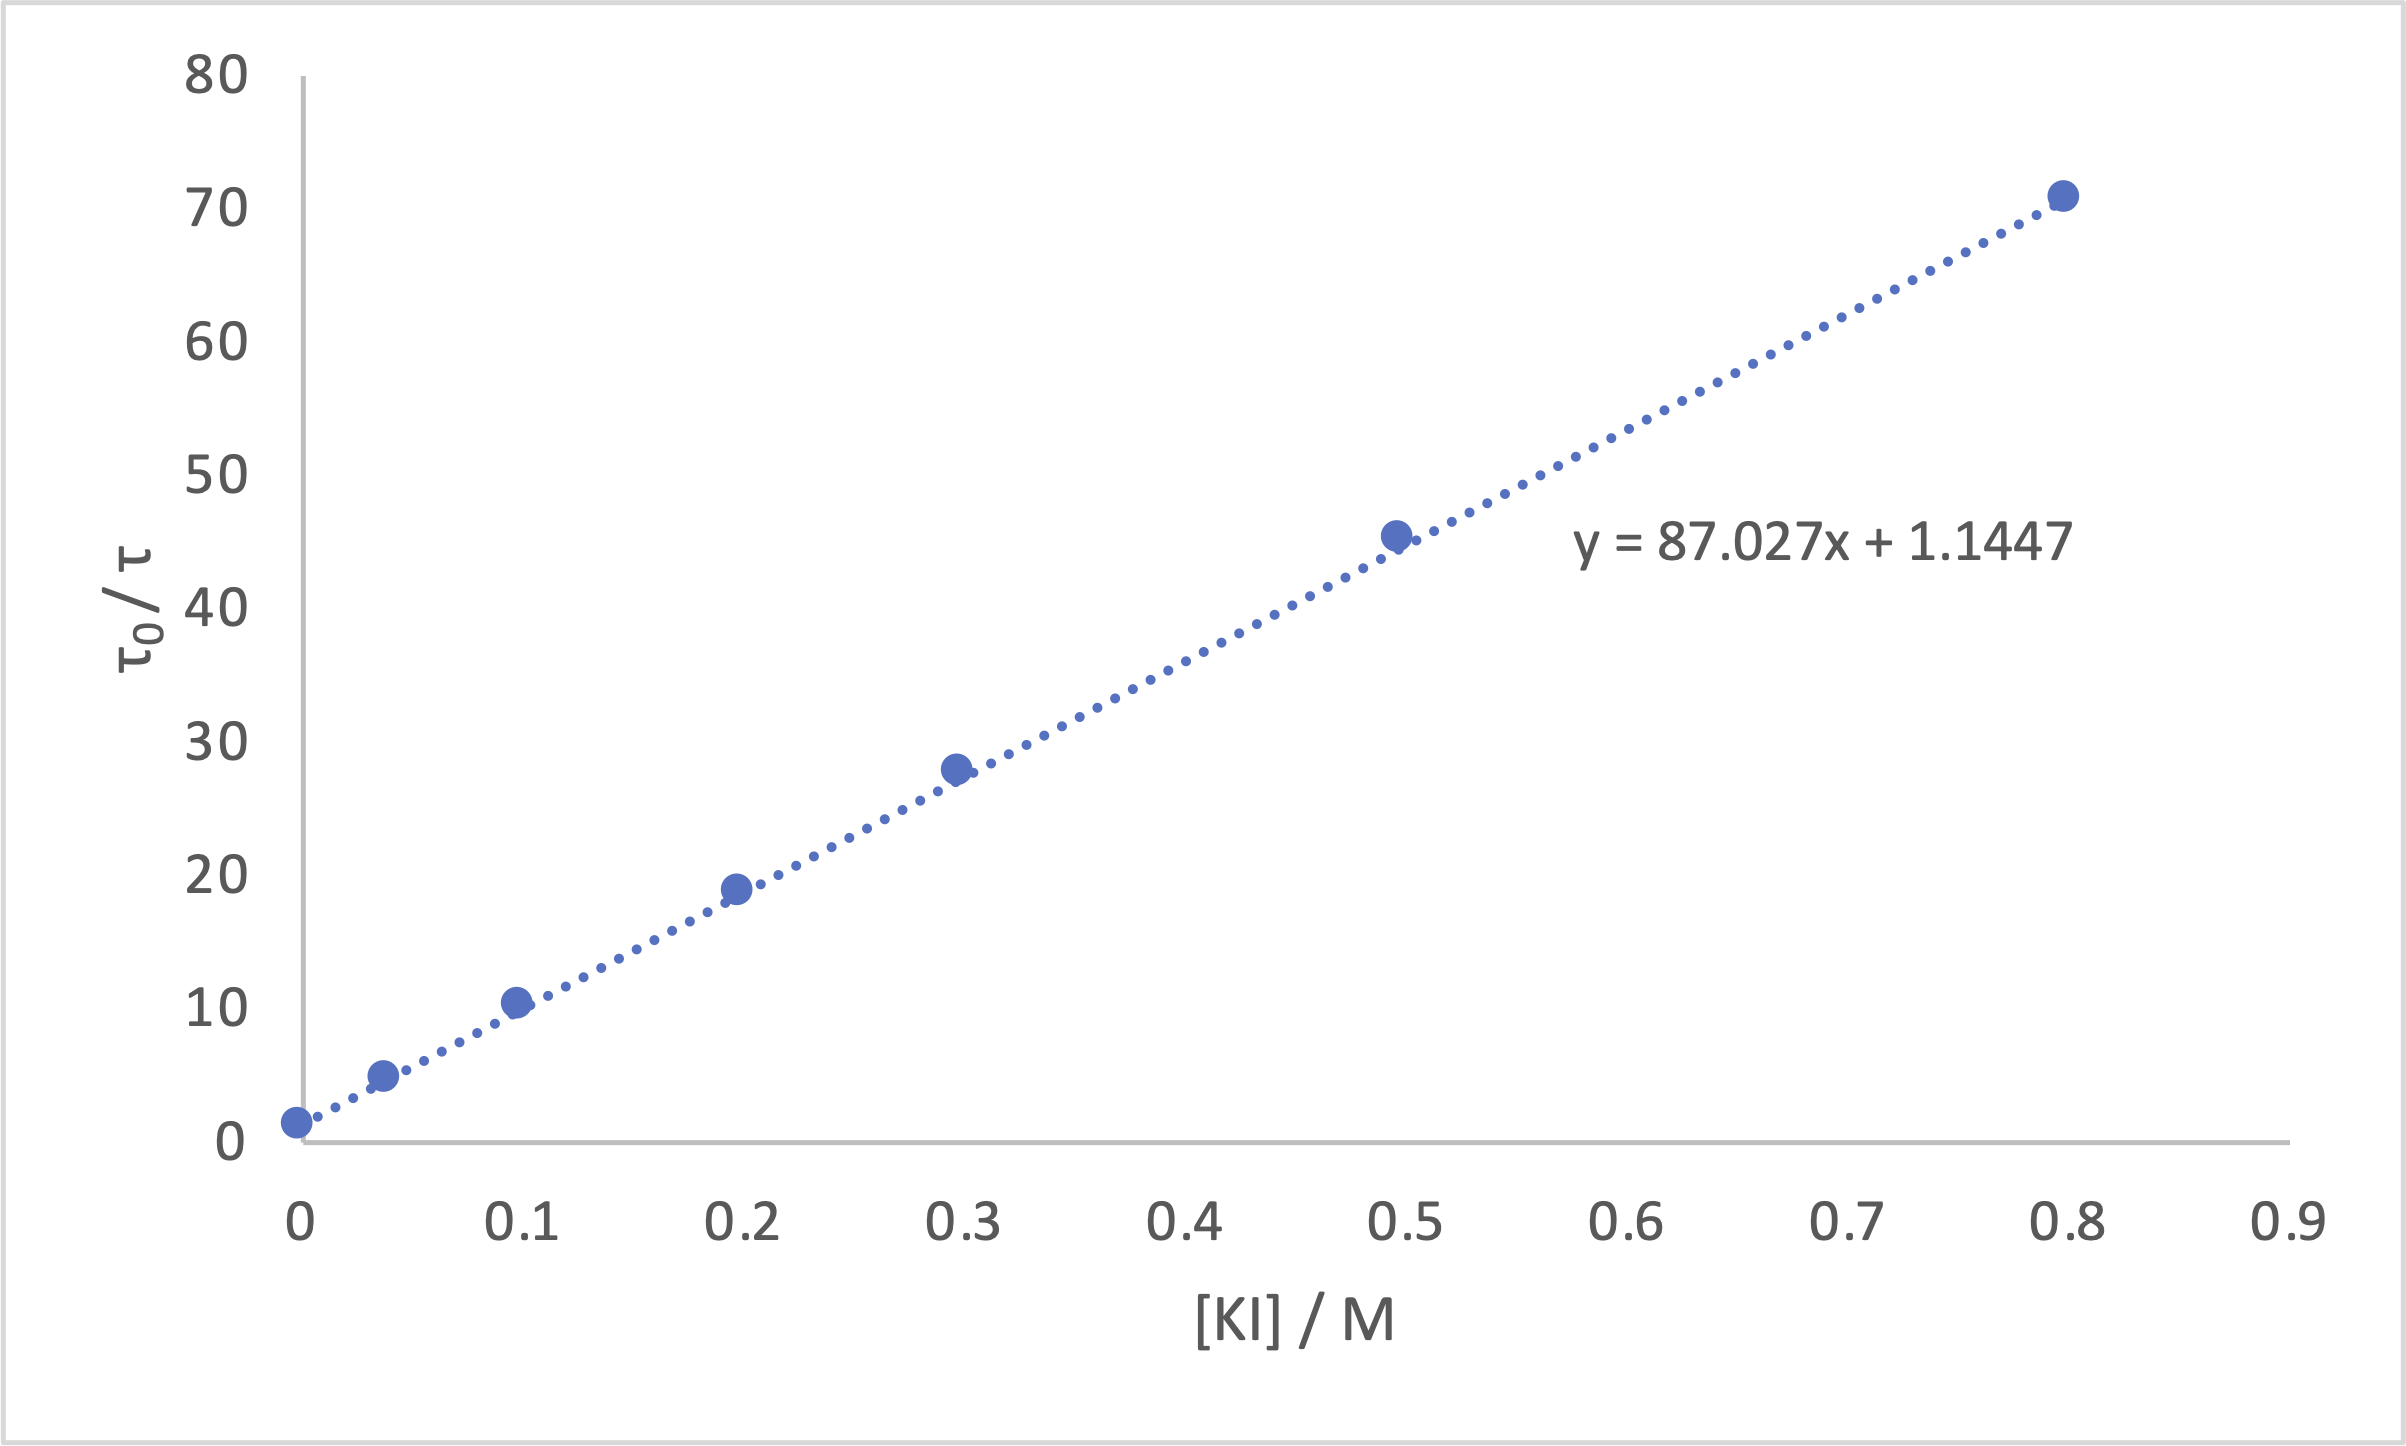
\includegraphics[width=0.7\linewidth]{images/graphexcel} 

}

\caption{The Stern-Volmer plot from the data above drawn in excel.}\label{fig:excel}
\end{figure}

\begin{figure}

{\centering 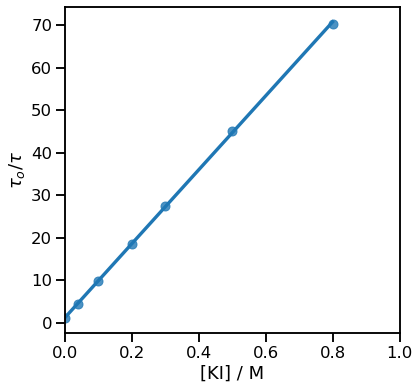
\includegraphics[width=0.5\linewidth]{images/graphpython} 

}

\caption{The Stern-Volmer plot from the data above drawn in python.}\label{fig:python}
\end{figure}

\hypertarget{sec:summary3}{%
\section{Summary of concepts learnt}\label{sec:summary3}}

\begin{itemize}
\tightlist
\item
  Units and any scaling factors should appear behind a solidus (/) not brackets.
\item
  Tables with headers work like equations, the horizontal bar works like a equals sign.
\item
  It should always be clear what is contained in a table - use square brackets for concentrations
\item
  Equations should be rearranged so they can be plotted in the form \(y=mx+c\).
\end{itemize}

When plotting graphs:

\begin{itemize}
\tightlist
\item
  the dependent variable (the thing you have control of or something related to it) goes on the horizontal \(x\)-axis.
\item
  the independent variable (the thing you measure or something related to it) goes on the vertical \(y\)-axis.
\item
  when plotting data data points should be used and they should not be connected by lines.
\item
  a line of best fit should be used when there is a mathematical reason to do so, so if plotting data as \(y=mx+c\) a straight line should be fitted.
\item
  you should never force a line of best fit through a given intercept.
\end{itemize}

\hypertarget{sec:Questions3}{%
\section{Questions}\label{sec:Questions3}}

When plotting graphs feel free to plot either by hand, in python, excel or numbers. The choice is entirely up to you.

\hypertarget{subsec:sketch}{%
\subsection{Sketch graphs}\label{subsec:sketch}}

Answers for these questions are in Section \ref{subsec:sketchans}.

For the following equations sketch suitable linear plots indicating values of the intercept and gradient on each sketch.

\begin{enumerate}
\def\labelenumi{\arabic{enumi}.}
\item
  Show how absorption, \(A\), changes with concentration, \(c\): \(A = \varepsilon c l\)
\item
  Show how pressure, \(p\), changes with temperature, \(T\): \(pV = nRT\)
\item
  Show how pressure, \(p\), changes with volume, \(V\): \(pV = nRT\)
\end{enumerate}

\hypertarget{subsec:2ndkintetics}{%
\subsection{Second order kinetics}\label{subsec:2ndkintetics}}

Answers for these questions are in Section \ref{subsec:2ndkinteticsans}.

Use the following table of data to plot a graph of \(\frac{1}{[A]}\) against t. Find the gradient and intercept.

(Just to note here you are plotting the equation \(\frac{1}{[A]}=\frac{1}{[A]_0}+kt\)).

\begin{longtable}[]{@{}cc@{}}
\toprule
t / s & 10\textsuperscript{4} {[}A{]} / mol dm\textsuperscript{-3}\tabularnewline
\midrule
\endhead
100 & 21.0\tabularnewline
200 & 12.0\tabularnewline
300 & 8.4\tabularnewline
400 & 7.1\tabularnewline
500 & 5.6\tabularnewline
\bottomrule
\end{longtable}

\hypertarget{subsec:clausius}{%
\subsection{Clausius-Clapeyron equation}\label{subsec:clausius}}

Answers for these questions are in Section \ref{subsec:arrheniusans}.

The relationship between the vapour pressure and temperature of diethyl ether (Table \ref{tab:ether}) can be modeled using the Clausius-Claeyron equation (Equation \eqref{eq:clausius}) to determine the enthalpy of vapourisation \(\Delta _{vap}H^\circ\).

\begin{equation}
\ln p = -\frac{\Delta_{vap}H^\circ}{RT}+C
\label{eq:clausius}
\end{equation}

\begin{enumerate}
\def\labelenumi{\arabic{enumi}.}
\tightlist
\item
  Determine \(\Delta _{vap}H^\circ\).
\item
  Determine the temperature diethyl ether boils at, at 1 atmosphere (760 mm Hg). \emph{Hint: determine C}
\end{enumerate}

\begin{longtable}[]{@{}cc@{}}
\caption{\label{tab:ether} The measured vapor pressure of ether (in mm Hg) at sub-zero temperatures.}\tabularnewline
\toprule
\(p\) / mm Hg & T / ºC\tabularnewline
\midrule
\endfirsthead
\toprule
\(p\) / mm Hg & T / ºC\tabularnewline
\midrule
\endhead
17 & -38\tabularnewline
28 & -30\tabularnewline
40 & -25\tabularnewline
55 & -20\tabularnewline
75 & -15\tabularnewline
97 & -10\tabularnewline
125 & -5\tabularnewline
157 & 0\tabularnewline
\bottomrule
\end{longtable}

\hypertarget{subsec:arrhenius}{%
\subsection{Arrhenius equation}\label{subsec:arrhenius}}

Answers for these questions are in Section \ref{subsec:arrheniusans}.

The Arrhenius equation (Equation \eqref{eq:arrhenius} shows how the rate of reaction, \(k\), depends upon the temperature of the reaction, \(T\)).

\begin{equation}
k=Ae^{-\frac{E_a}{RT}}
\label{eq:arrhenius}
\end{equation}

For the data shown in Table \ref{tab:arrhenius} plot an appropriate linear plot in order to determine the activation energy, \(E_a\), and the pre-exponential factor, \(A\).

\begin{longtable}[]{@{}cc@{}}
\caption{\label{tab:arrhenius} The variation of measured rate constant with temperature for an undergraduate's experiment.}\tabularnewline
\toprule
T / ºC & k / 10\textsuperscript{5} s\textsuperscript{-1}\tabularnewline
\midrule
\endfirsthead
\toprule
T / ºC & k / 10\textsuperscript{5} s\textsuperscript{-1}\tabularnewline
\midrule
\endhead
283 & 0.000352\tabularnewline
356 & 0.0302\tabularnewline
393 & 0.219\tabularnewline
427 & 1.16\tabularnewline
508 & 39.5\tabularnewline
\bottomrule
\end{longtable}

\hypertarget{sec:Answers3}{%
\section{Answers}\label{sec:Answers3}}

\hypertarget{subsec:sketchans}{%
\subsection{Sketch graphs}\label{subsec:sketchans}}

\begin{enumerate}
\def\labelenumi{\arabic{enumi}.}
\item
\end{enumerate}

\begin{figure}

{\centering 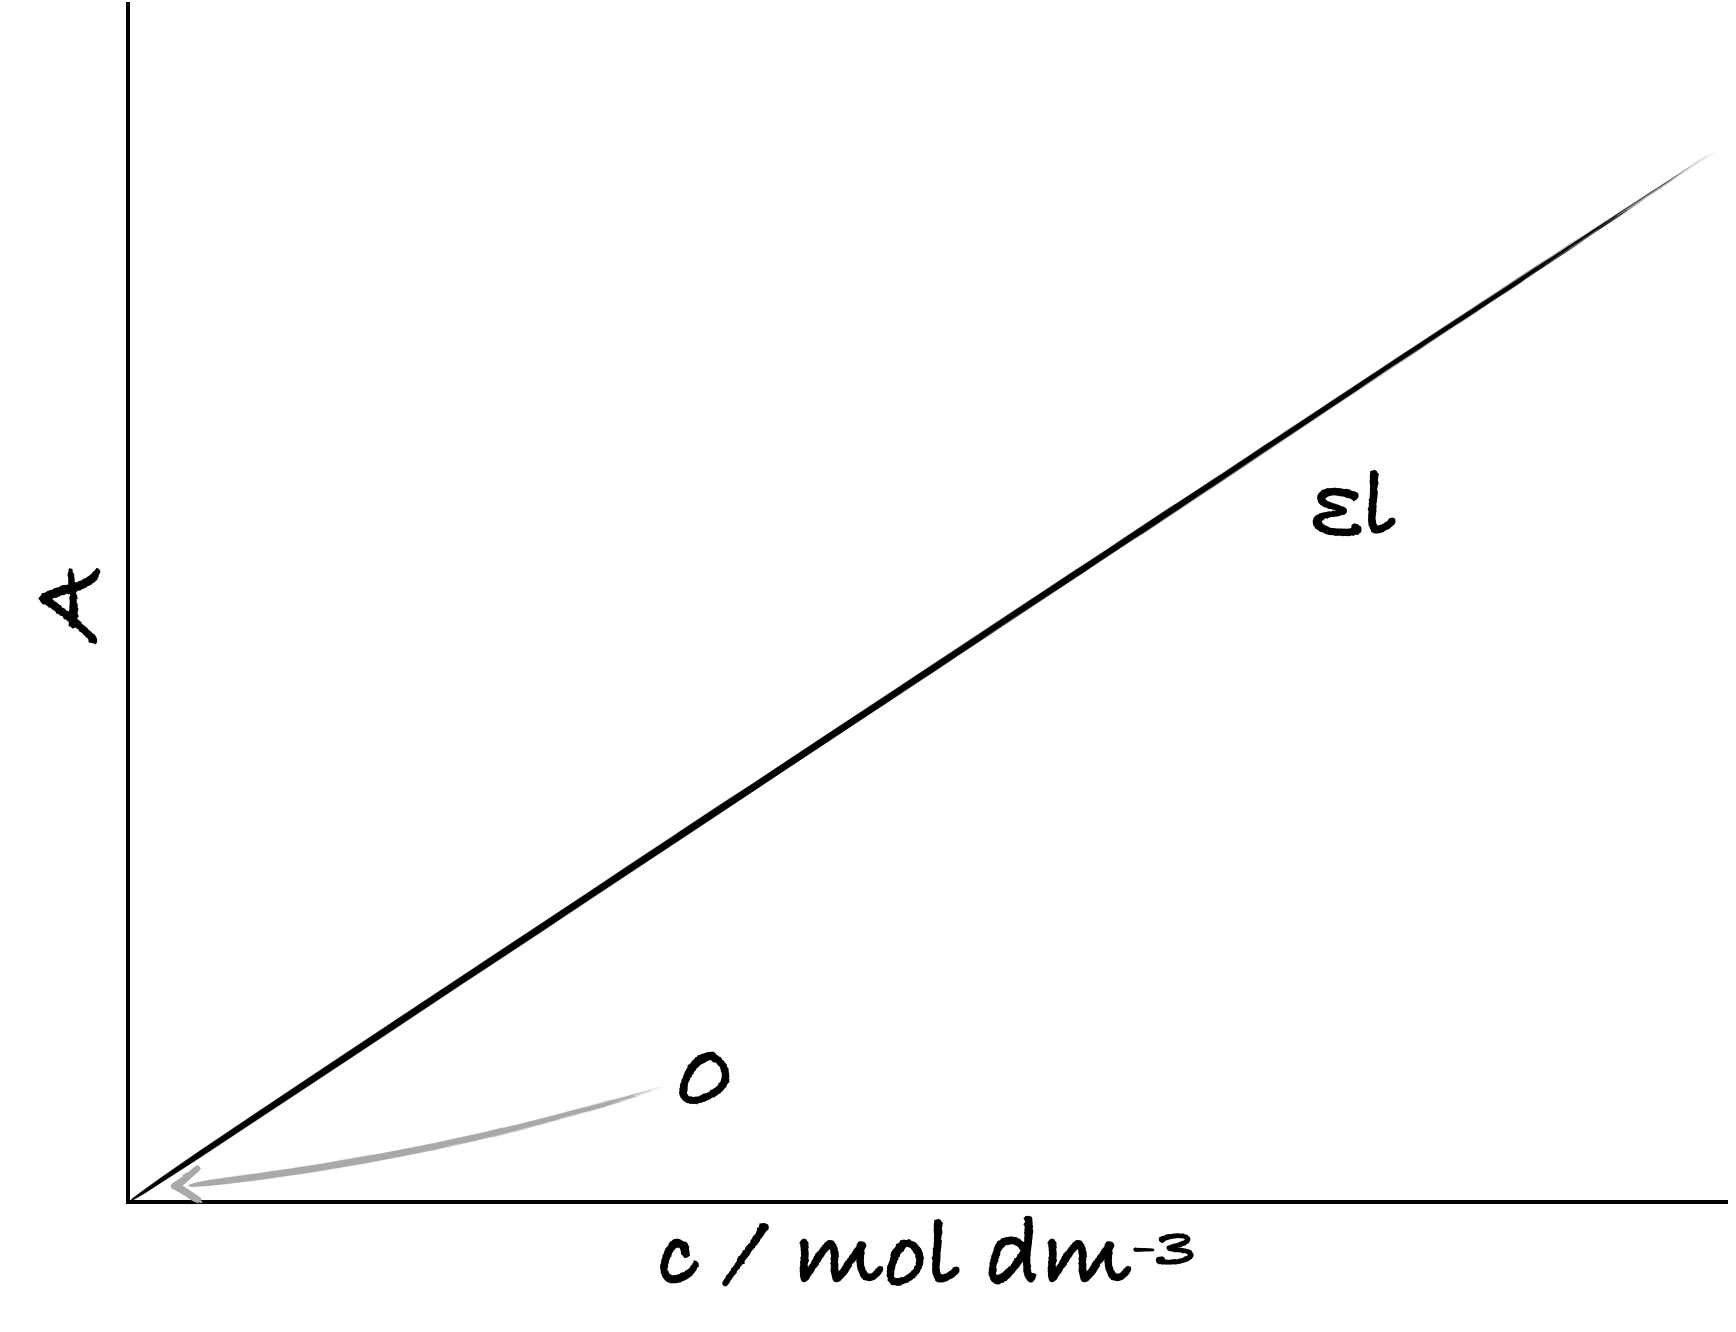
\includegraphics[width=0.3\linewidth]{images/abssketch} 

}

\caption{The Beer-Lambert relationship to show how absorbance, the dependent variable, changes with concentration, the independent variable.}\label{fig:abs}
\end{figure}

\begin{enumerate}
\def\labelenumi{\arabic{enumi}.}
\setcounter{enumi}{1}
\item
\end{enumerate}

\begin{figure}

{\centering 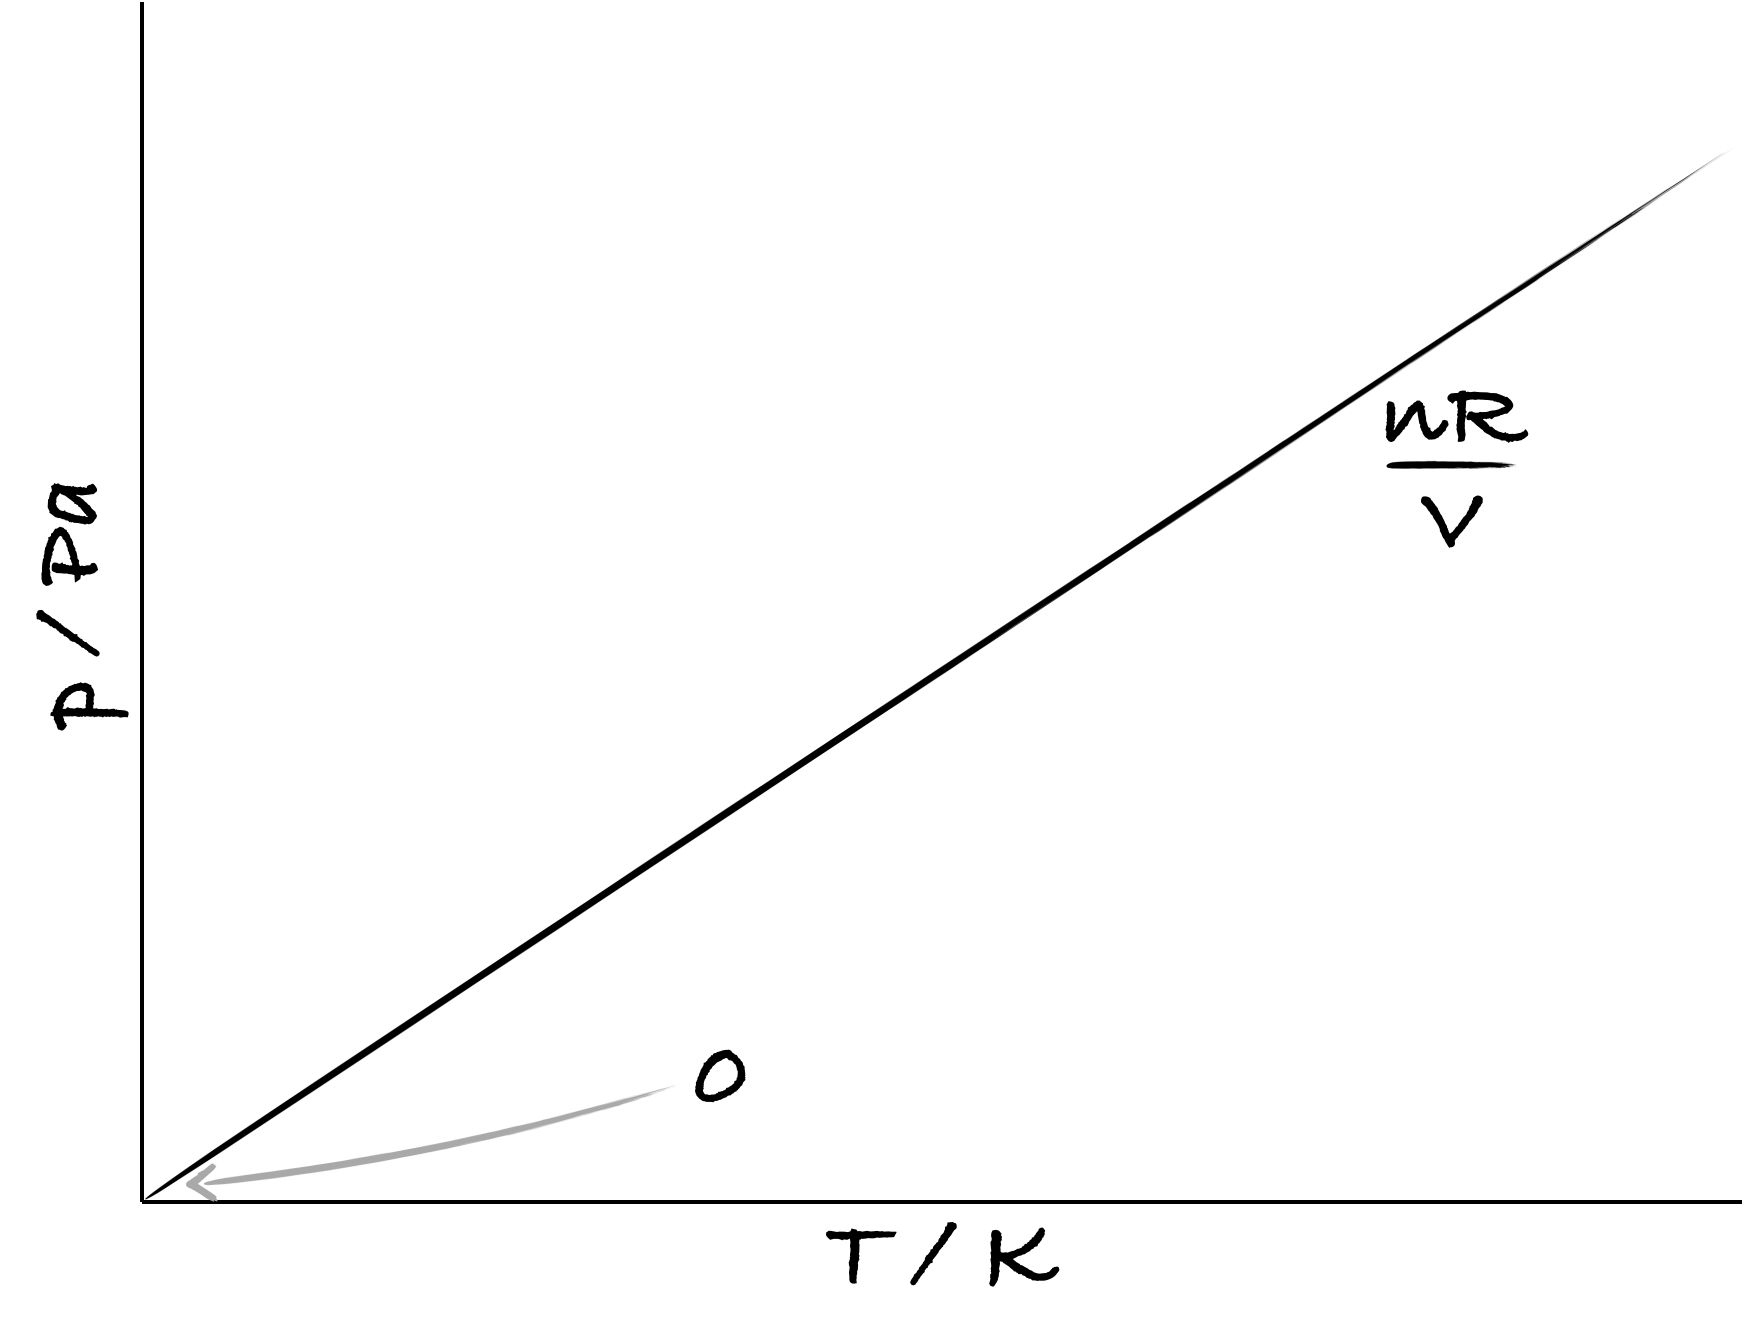
\includegraphics[width=0.3\linewidth]{images/pTsketch} 

}

\caption{A sketch to show how the pressure of an ideal gas, the dependent variable,changes with temperature, the independent variable.}\label{fig:pT}
\end{figure}

\begin{enumerate}
\def\labelenumi{\arabic{enumi}.}
\setcounter{enumi}{2}
\item
\end{enumerate}

\begin{figure}

{\centering 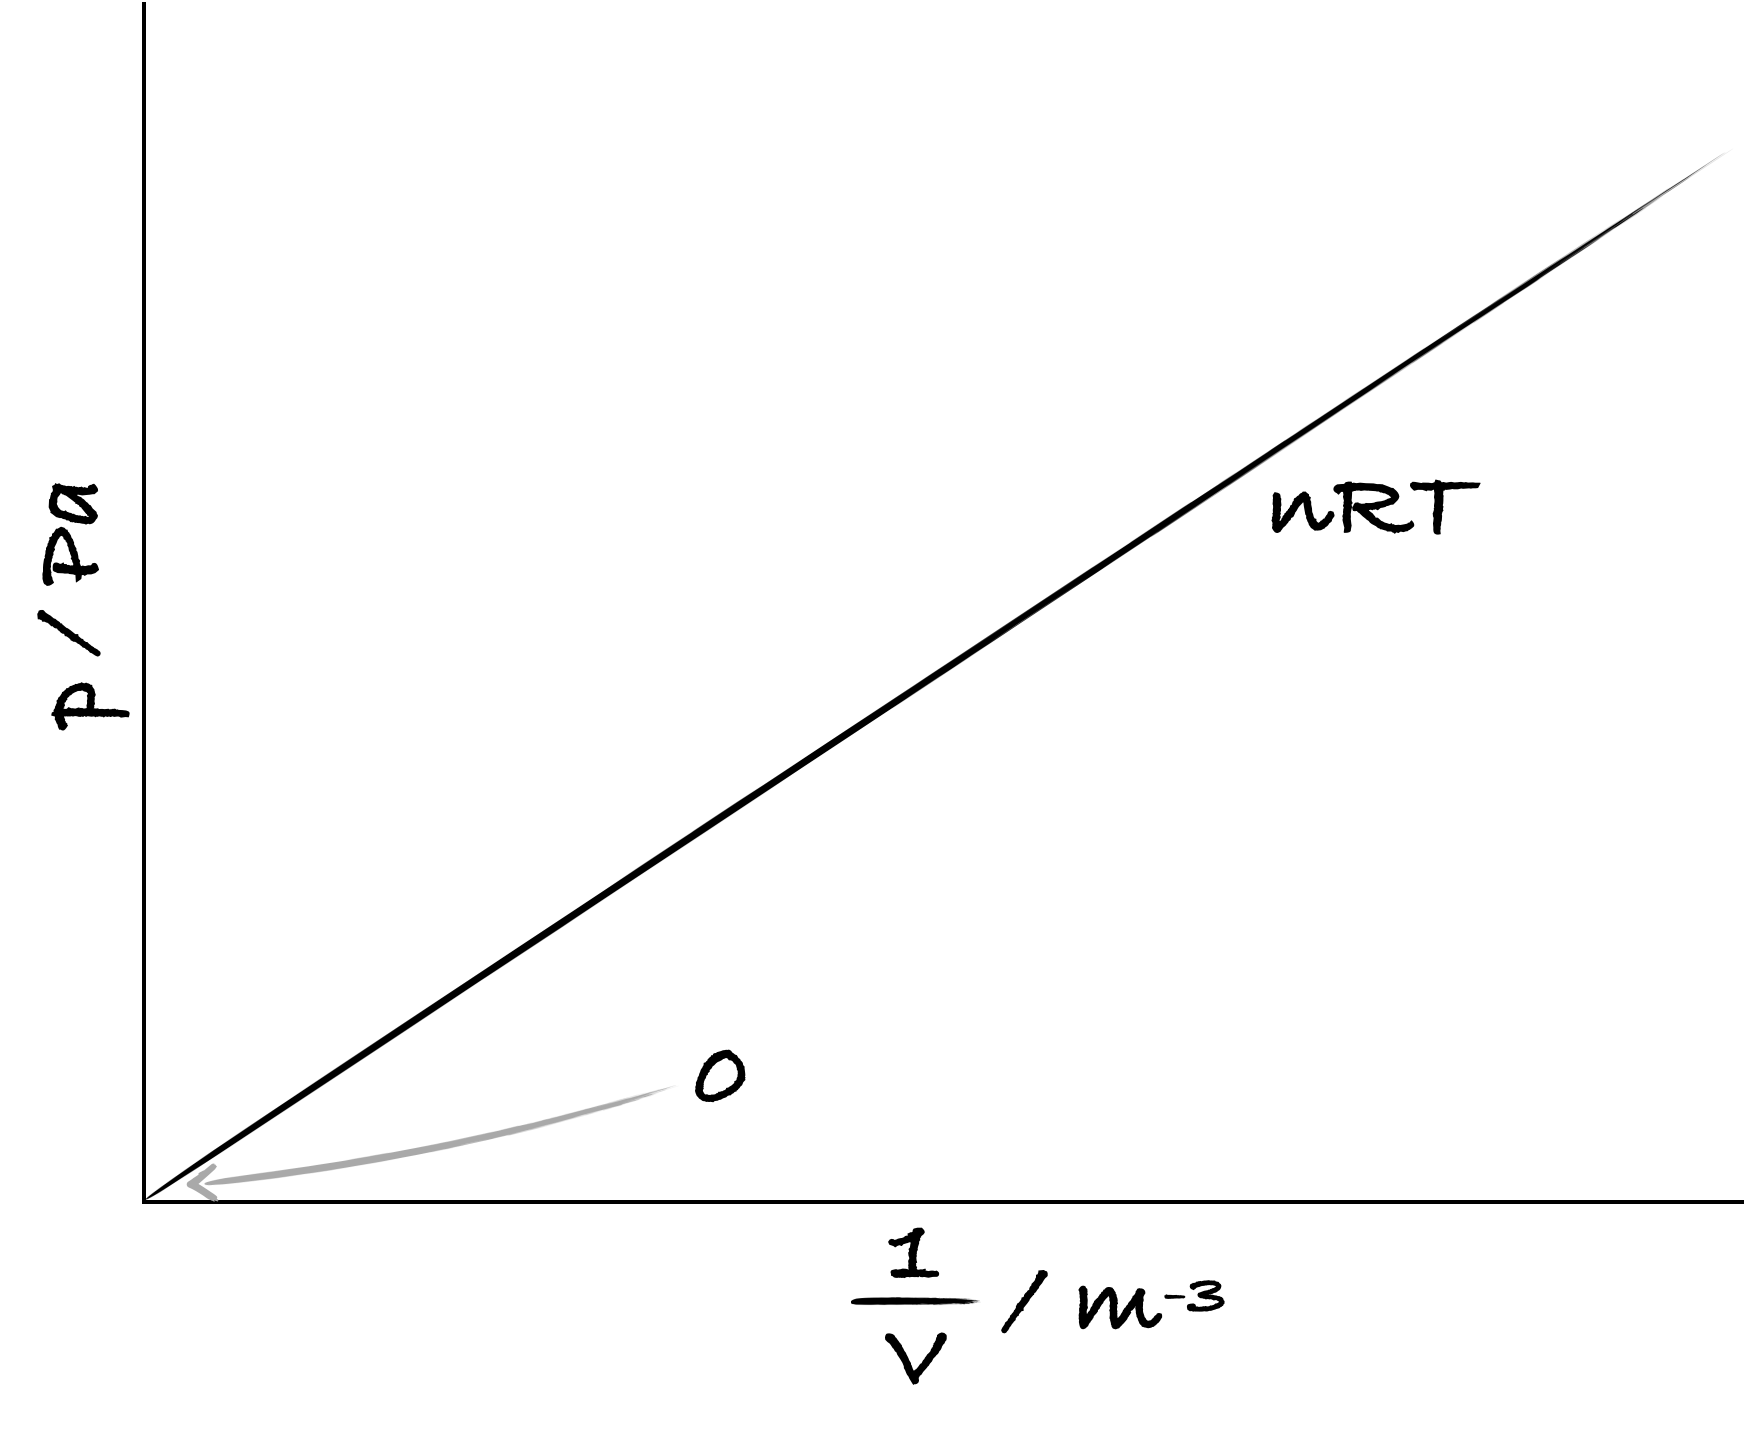
\includegraphics[width=0.3\linewidth]{images/pVsketch} 

}

\caption{A sketch to show how the pressure of an ideal gas, the dependent variable,changes with volume, the independent variable - note for a linear relationship we have 1/V on the x-axis.}\label{fig:pV}
\end{figure}

\hypertarget{subsec:2ndkinteticsans}{%
\subsection{Second order kinetics}\label{subsec:2ndkinteticsans}}

m = 3.19 M\textsuperscript{-1} s\textsuperscript{-1}, c = 180 M\textsuperscript{-1} ({[}A{]}\textsubscript{0} = 5.56 mM)

\hypertarget{subsec:clausiusans}{%
\subsection{Clausius-Clapeyron equation}\label{subsec:clausiusans}}

\(\Delta _{vap}H^\circ\) = 31.6 kJ mol\textsuperscript{-1}, 39 ºC.

\hypertarget{subsec:arrheniusans}{%
\subsection{Arrhenius equation}\label{subsec:arrheniusans}}

m = -22.4 × 10\textsuperscript{3} K, c = 43.7, \(E_a\) = 186 kJ mol\textsuperscript{-1}, \(A\) = 9.7 × 10\textsuperscript{18} s\^{}-1

\hypertarget{ch:Workshop4}{%
\chapter{Week 4}\label{ch:Workshop4}}

\hypertarget{sec:Prelim4}{%
\section{Preliminary infomation}\label{sec:Prelim4}}

Rates of change are important, whether it is the steepness of a hill (the rate of change of elevation with horizontal distance travelled), speed (rate of change of distance with time) or the rate of reaction (change in concentration of a reactant with respect to time). Differentiation is a mathematical method for determining the rate of change of one variable with another.

Some functions are `linear' (figure \ref{fig:linear}), and the rate of change of the function is the gradient, \(\frac{\Delta y}{\Delta x}\). So if we look at figure \ref{fig:linear} the change of distance (\(\Delta y\)) with respect to time (\(\Delta x\)) is just the gradient, but not all functions are linear, and so not all gradients are constant, therefore not all rates of change are constant.

\begin{figure}

{\centering 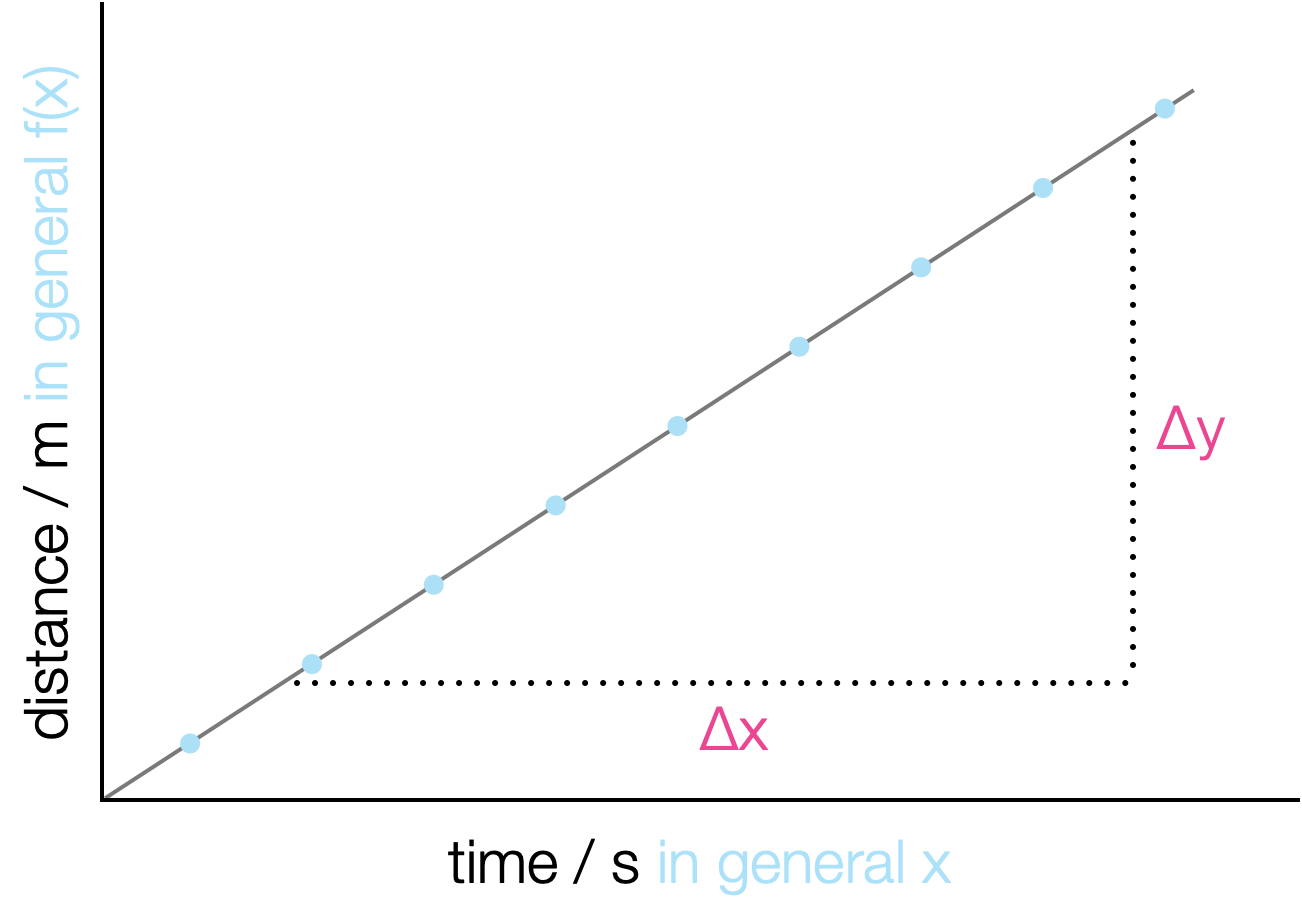
\includegraphics[width=0.5\linewidth]{images/linearplot} 

}

\caption{A linear plot with time on the x-axis and distance on the y axis, the gradient of the line is the velocity, the rate of change of distance with respect to time.}\label{fig:linear}
\end{figure}

Many chemical reactions show a curved decay of concentration of reactant with time (figure \ref{fig:expplot}). In this case the gradient of the line depends on where you measure it.

\begin{figure}

{\centering 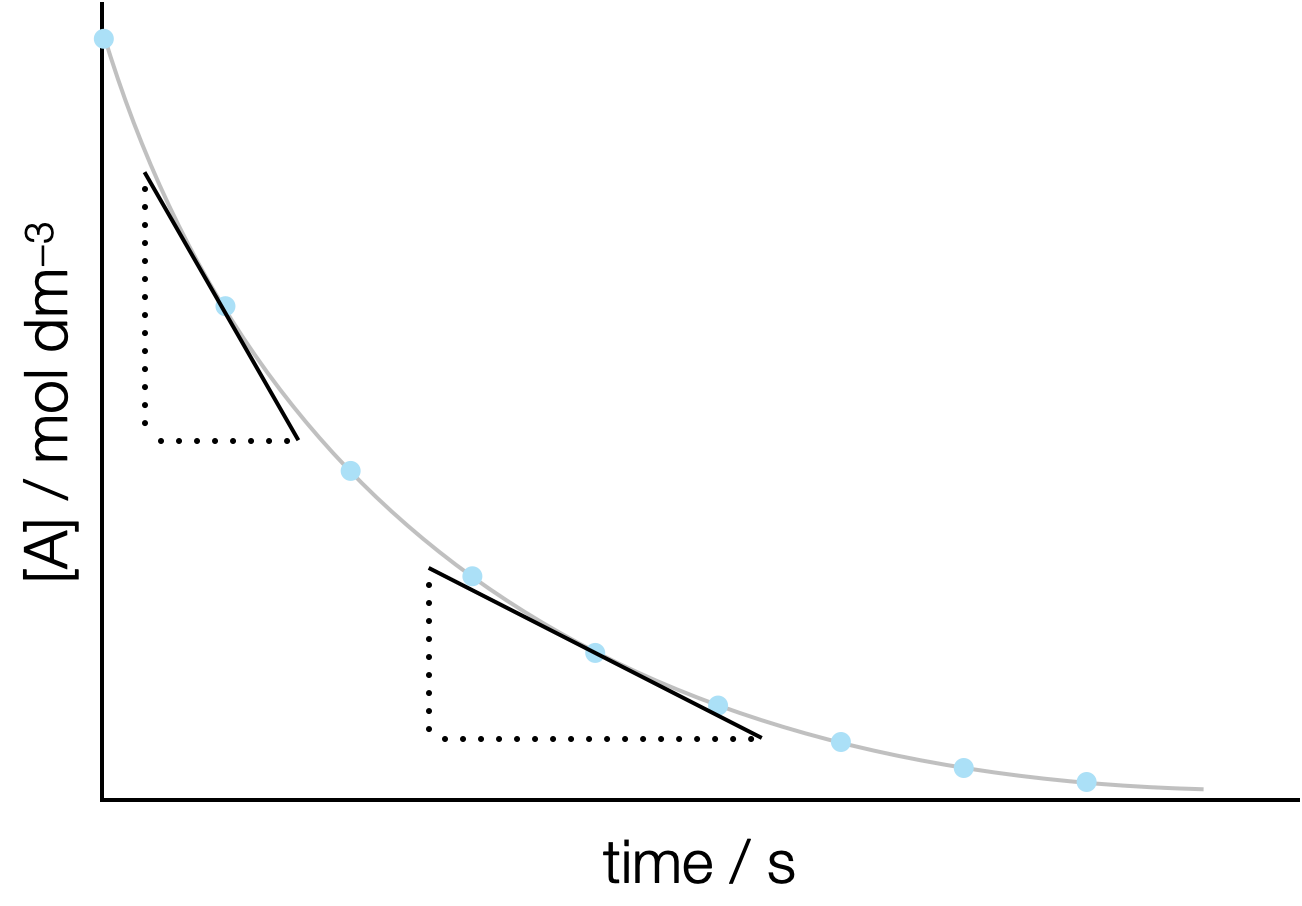
\includegraphics[width=0.5\linewidth]{images/expplot} 

}

\caption{An exponential decay plot with time on the x-axis and concentration of a reactant A on the y axis, the gradient is the rate of reaction and the rate of reaction varies with how far the reaction has proceeded.}\label{fig:expplot}
\end{figure}

Differentiation is a mathematical way of determining what this gradient is at any given point.

\hypertarget{subsec:whatisdiff}{%
\subsection{What is differentiation}\label{subsec:whatisdiff}}

If we look at figure \ref{fig:linear} the line fits the equation \(y = mx+c\). The gradient of that line, \(m\), is given by the change in y divided by the change in x:

\begin{equation*}
m = \frac{\Delta y}{\Delta x} = \frac{y_2-y_1}{x_2-x_1}
\end{equation*}

For each of the two points used to determine the gradient we may write an equation defining that point:

\begin{equation*}
y_1 = mx_1 + c\\
y_2 = mx_2 + c
\end{equation*}

and \(x_2 = x_1+\Delta x\)

and so we can express \(y_2\) as:

\begin{equation*}
y_2 = m(x_1+ \Delta x) + c
\end{equation*}

The gradient of this line is:

\begin{equation*}
 \frac{\Delta y}{\Delta x} = \frac{y_2-y_1}{x_2-x_1}=\frac{(m(x_1+ \Delta x) + c) - (mx_1 + c)}{\Delta x} = m\frac{\Delta x}{\Delta x}=m
\end{equation*}

This is the least surprising result (and a relatively large amount of work) that you will likely see, but this principle can be used to show \emph{what} differentiation is.

We can now show this same idea for a more complicated function, for example a quadratic.

\hypertarget{showing-why-the-differential-of-a-quadratic-is-a-linear-function-of-x}{%
\subsection{Showing why the differential of a quadratic is a linear function of x}\label{showing-why-the-differential-of-a-quadratic-is-a-linear-function-of-x}}

\begin{figure}

{\centering 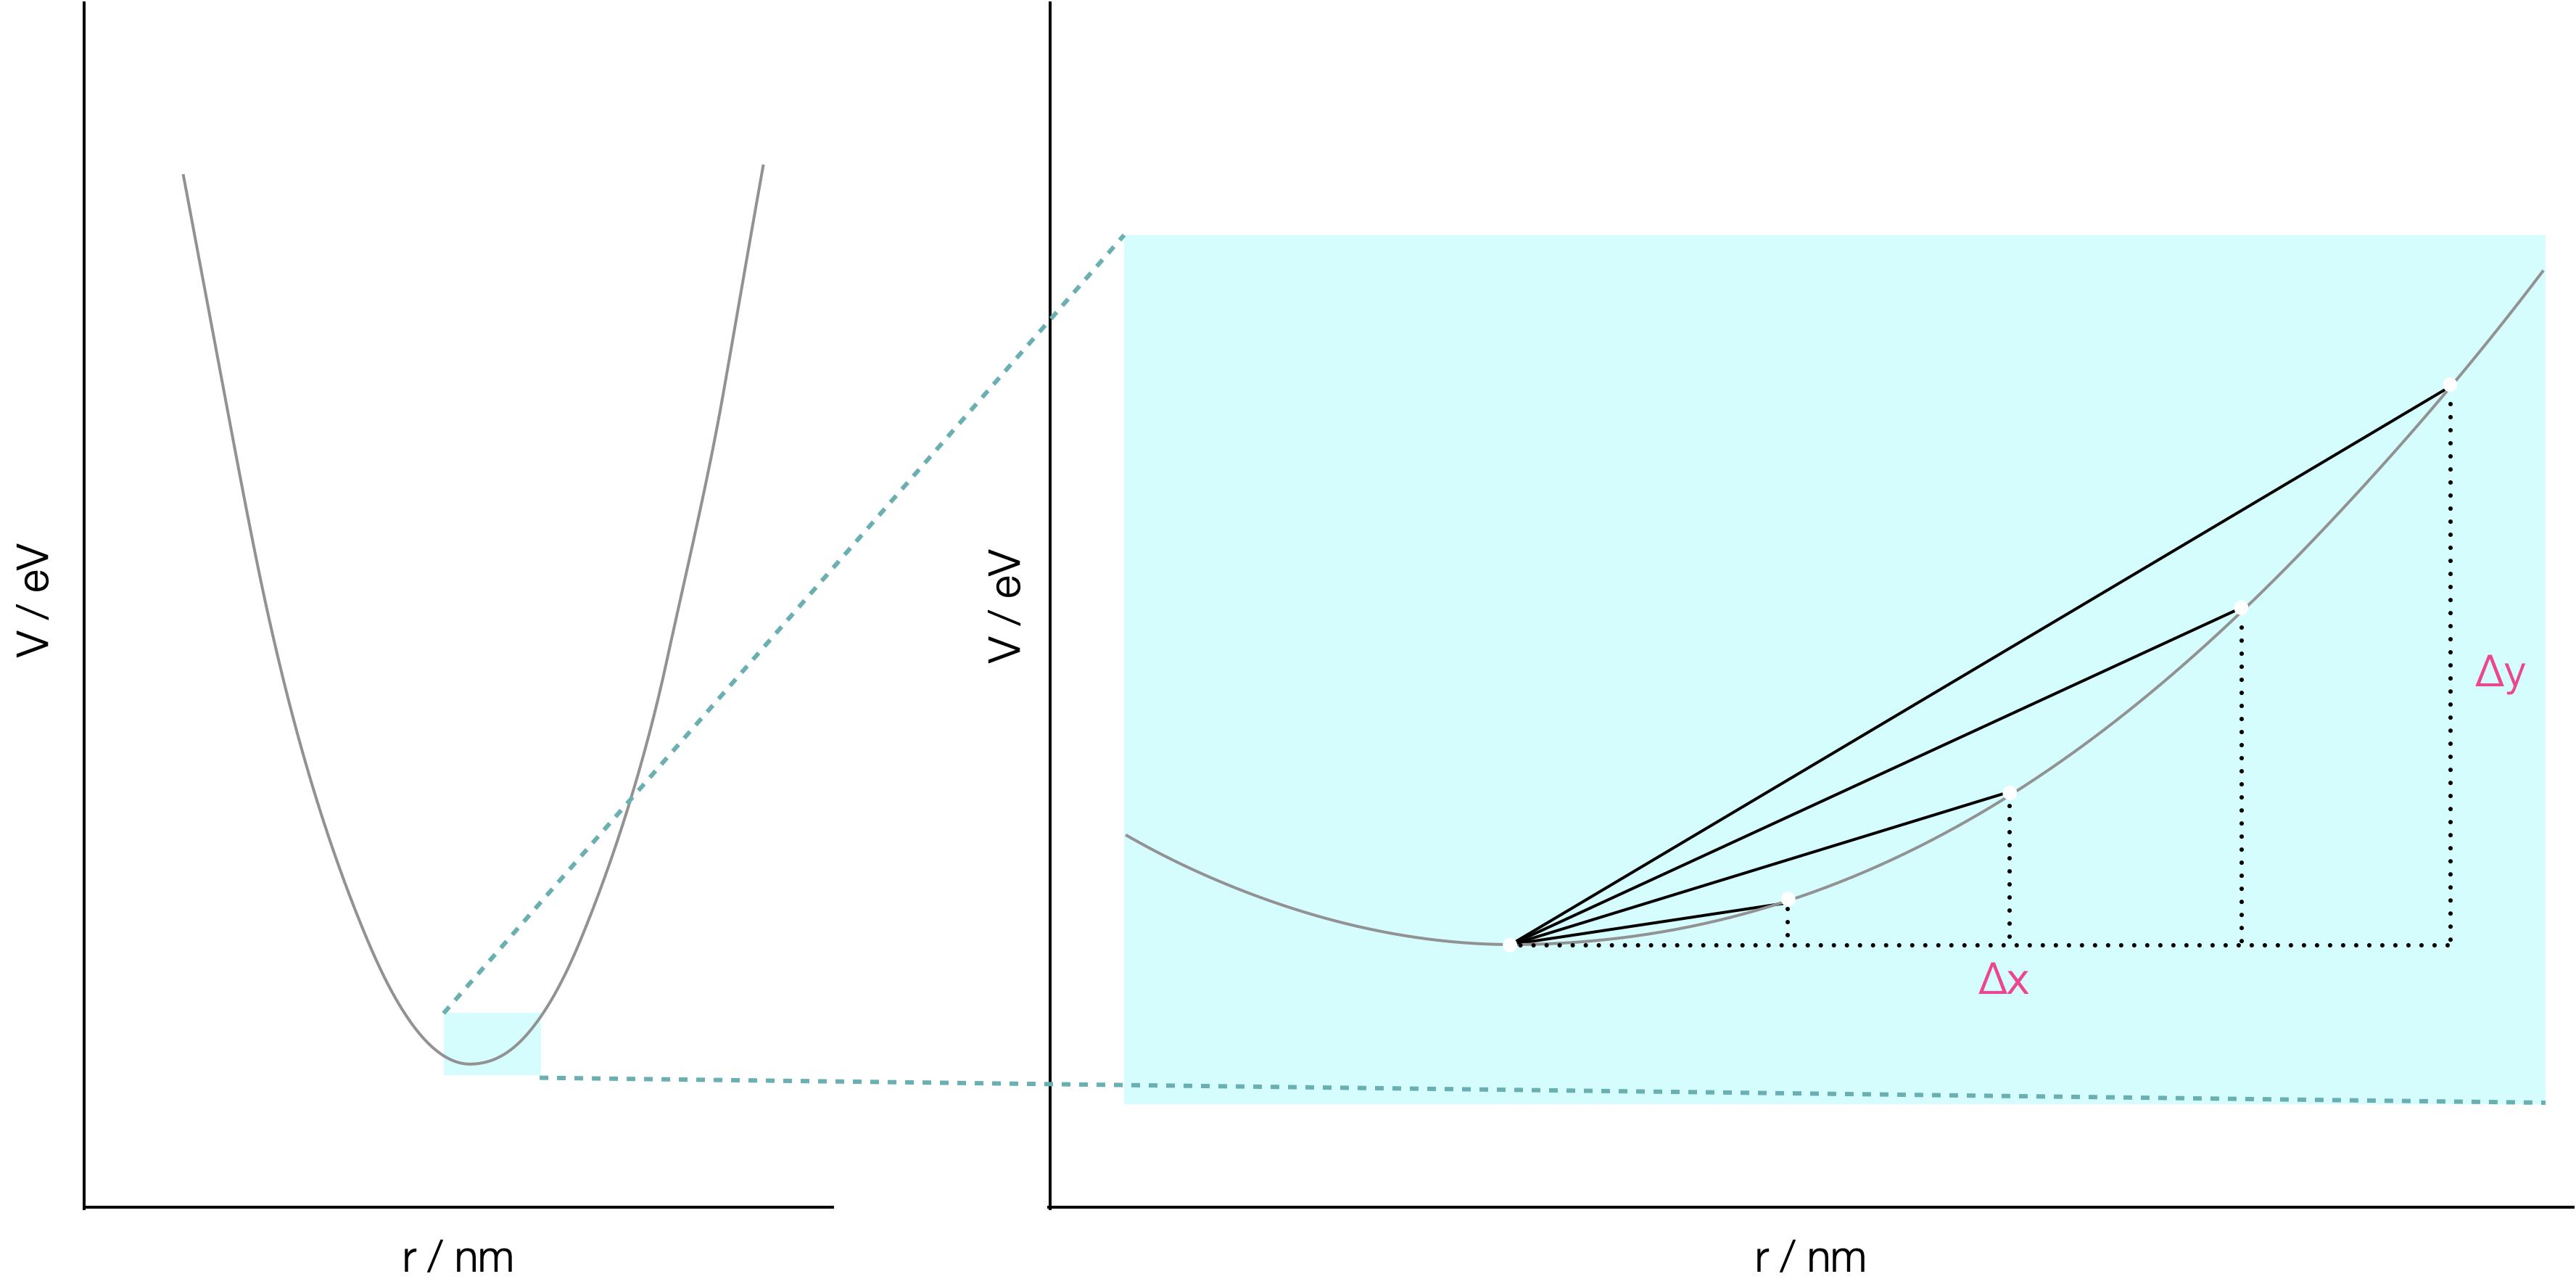
\includegraphics[width=0.8\linewidth]{images/quadratic} 

}

\caption{Left: a harmonic oscillator model showing quadratic behaviour. Right: a zoomed in section of this model, showing different values of the gradient for different values of Δx, the smaller the value of Δx the better approximation to the gradient.}\label{fig:quad}
\end{figure}

Figure \ref{fig:quad} shows a harmonic oscilator which is a quadratic function of the form \(y=ax^2+bx+c\). The image shows that the gradient of the point at the bottom of the curve may be approximated by different gradient triangles, the smaller the triangle the better the approximation to the curve, and therefore the better the approximation of the gradient at that point. As these triangles get smaller they better approach the gradient of the tangent to the line.

We can determine the gradient of of any point \((x_0, y_0)\), by using a second point \((x_1, y_1)\) as we did in section \ref{subsec:whatisdiff}.

If a quadratic has the general form \(y=ax^2+bx+c\), then we can write the equations for the points \((x_0, y_0)\) and \((x_1, y_1)\).

\begin{equation*}
y_0 = ax_0^2+bx_0+c\\
y_1 = ax_1^2+bx_1+c
\end{equation*}

and we know that \(x_1=x_0+\Delta x\), so we can rewrite the equation for \(y_1\):

\begin{equation*}
y_0 = ax_0^2+bx_0+c\\
y_1 = a(x_0+\Delta x)^2+b(x_0+\Delta x)+c
\end{equation*}

However as this gradient triangle reduces in size we can use a lower case delta (\(\delta\)) to indicate just a very small change in the x \& y values.

\begin{equation*}
y_0 = ax_0^2+bx_0+c\\
y_1 = a(x_0+\delta x)^2+b(x_0+\delta x)+c
\end{equation*}

The gradient of this line is given by:

\begin{equation*}
\frac{\delta y}{\delta x} = \frac{y_1-y_0}{x_1-x_0} = \frac{(a(x_0+\delta x)^2+b(x_0+\delta x)+c)-(ax_0^2+bx_0+c)}{\delta x}
\end{equation*}

Simplifying:

\begin{equation*}
\frac{\delta y}{\delta x} = \frac{2ax_0 \delta x +2a \delta x^2+b\delta x}{\delta x}
\end{equation*}

With cancelling:

\begin{equation*}
\frac{\delta y}{\delta x} = 2ax_0+2a \delta x+b
\end{equation*}

As the size of the gradient triangle reduces (or more formally as \(\delta x \rightarrow 0\)) then the term with the remaining \(\delta x\) tends to zero. When we do this we use the terminology \(\frac{\textrm{d}y}{\textrm{d}x}\) to denote that we have reduced the size of this step to zero (an entirely mathematical concept). The formal notation of this is: \(\frac{\textrm{d}y}{\textrm{d}x}=\lim\limits_{x \to 0}\frac{\delta y}{\delta x}\), our differential \(\frac{\textrm{d}y}{\textrm{d}x}\) is what we get when we reduce the size of our step between our two values used to determine the gradient to zero.

So:
\begin{equation*}
\frac{\textrm{d}}{\textrm{d}x} ax^2+bx+c = 2ax+b
\end{equation*}

This is differentiation, and instead of going through this process with every possible function we can learn the rules of differentiation so that we can quickly get to the result of most functions that we can think of.

\hypertarget{notation-of-differentiation}{%
\subsection{Notation of differentiation}\label{notation-of-differentiation}}

There are a couple of different ways of noting differentials, I tend to use a mixture of two methods. There are two different methods of reporting functions firstly where \(y\) is a function of \(x\) (\emph{e.g.} \(y = ax^2+bx+c\)) where the differential notation \(\frac{\textrm{d}y}{\textrm{d}x}\) tends to be used, secondly where we have a function of \(x\) (\emph{e.g.} \(f(x) = ax^2+bx+c\)) where the differential notation \(f'(x)\) tends to be used.

We can also differentiate functions more than once, if we differentiate a function twice with respect to \(x\) we can use either the notation \(\frac{\textrm{d}^2y}{\textrm{d}x^2}\) or \(f''(x)\).

The reasons why we may wish to differentiate a function twice are explained in section \ref{subsec:turningpoints}

\hypertarget{subsec:diffconst}{%
\subsection{Differentiating constants}\label{subsec:diffconst}}

Graphically we can imagine a constant as a horizontal line on a graph, no matter the value of x, a constant is just that a constant, and therefore it should come as no surprise that the differential of a constant, \(c\) is 0. Formally:

\begin{equation}
y = c\\
\frac{\textrm{d}y}{\textrm{d}x}=0
\label{eq:diffconst}
\end{equation}

Recall that anything raised to the power 0 is one, so if we differentiate anything raised to the power zero we get 0.

\hypertarget{subsec:diffpolynomial}{%
\subsection{Differentiating polynomials}\label{subsec:diffpolynomial}}

When differentiating polynomials the rule is always the same for all numerical powers except \(x^0\) (a constant). In this case we multiply our variable by the old power, and deduct one from the starting power. So, if \(a\) and \(b\) are constants:

\begin{equation}
y = ax^b\\
\frac{\textrm{d}y}{\textrm{d}x}=abx^{b-1}\\
\textrm{when } x \neq 0
\label{eq:diffpoly}
\end{equation}

This is true for positive intergers:

\(y = 3x^3\) \(\frac{\textrm{d}y}{\textrm{d}x} = 9x^2\)

Negative integers (recall that negative powers are a way of expressing 1 over positive powers):
\(y = ax^{-3}\) \(\frac{\textrm{d}y}{\textrm{d}x} = -3ax^{-4}\)

and fractions:
\(y = 2x^{\frac{1}{2}}\) \(\frac{\textrm{d}y}{\textrm{d}x} = x^{-\frac{1}{2}}\)

Note in each case we have reduced the power by one, and multiplied the whole term by the old power.

\hypertarget{subsec:diffexp}{%
\subsection{Differentiating exponentials}\label{subsec:diffexp}}

\begin{equation}
y = be^{ax}\\
\frac{\textrm{d}y}{\textrm{d}x}=abe^{ax}
\label{eq:diffexp}
\end{equation}

Exponential functions may be expressed as a polynomial series (Section \ref{subsec:macexp}), this explains the result, but as chemists only the result of the differentiation is usually important.

For example if \(y=e^{-2x}\), then:

\begin{equation*}
\frac{\textrm{d}y}{\textrm{d}x}=-2e^{-2x}\\
\textrm{and:}\\
\frac{\textrm{d}^2y}{\textrm{d}x^2}=4e^{-2x}
\end{equation*}

\emph{Note how the power in an exponential function does not change.}

\hypertarget{subsec:difflogs}{%
\subsection{\texorpdfstring{Differentiating natural logs (\(\ln\))}{Differentiating natural logs (\textbackslash ln)}}\label{subsec:difflogs}}

We cannot directly differentiate any logs other than natural logs (\(\ln\)). We can use one of our rules of logs (equation \eqref{eq:convpower}) to convert the log to any other base to a natural log. However, natural logs describe behaviours found naturally in nature, such as chemical reactions and so it is rare to have to differentiate any other logs.

\begin{equation}
y = \ln {ax}\\
\frac{\textrm{d}y}{\textrm{d}x}=\frac{1}{x}
\label{eq:diffln}
\end{equation}

It may at first seem surprising that the constant \(a\) in equation \eqref{eq:diffln} disappears in the differential, however, if we think about our rules of logs (equation \eqref{eq:logadd}), then \(y=\ln {ax}\) may be rewritten as \(y = \ln a +\ln x\) and of course \(\ln a\) is a constant and so differentiates to 0 as shown in \eqref{eq:diffconst}.

\hypertarget{subsec:difftrig}{%
\subsection{Differentiating trig functions}\label{subsec:difftrig}}

If we look at how how the trig functions \(\sin\) and \(\cos\) vary (figure \ref{fig:trigcyclic}), we can see that when \(\sin x\) has a maximum value (at \(\frac{\pi}{2}\)) the gradient at that point is 0. We can also see that the value of \(\cos x\) at \(\frac{\pi}{2}\) is also 0, this isn't coincidence, the functions \(\sin\) and \(\cos\) are intrinsically linked.

\begin{figure}

{\centering 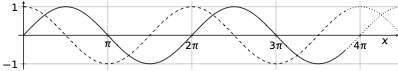
\includegraphics[width=0.8\linewidth]{images/trigcyclic} 

}

\caption{A plot of sin (x) (solid line) and cos (x) (dashed line) showing the repeating nature of the functions over 2π. We can note that when sin (x) reaches a maximum at π/2 and a minimum at 3π/2 (and the gradient is zero) then cos (x) is 0.}\label{fig:trigcyclic}
\end{figure}

In fact if we differentiate \(\sin x\) with respect to \(x\) we get \(\cos x\). You can see this if you look at the Maclaurin expansion for \(\sin\) (equation \eqref{eq:macsin}) and \(\cos\) (equation \eqref{eq:maccos}).

\begin{figure}

{\centering 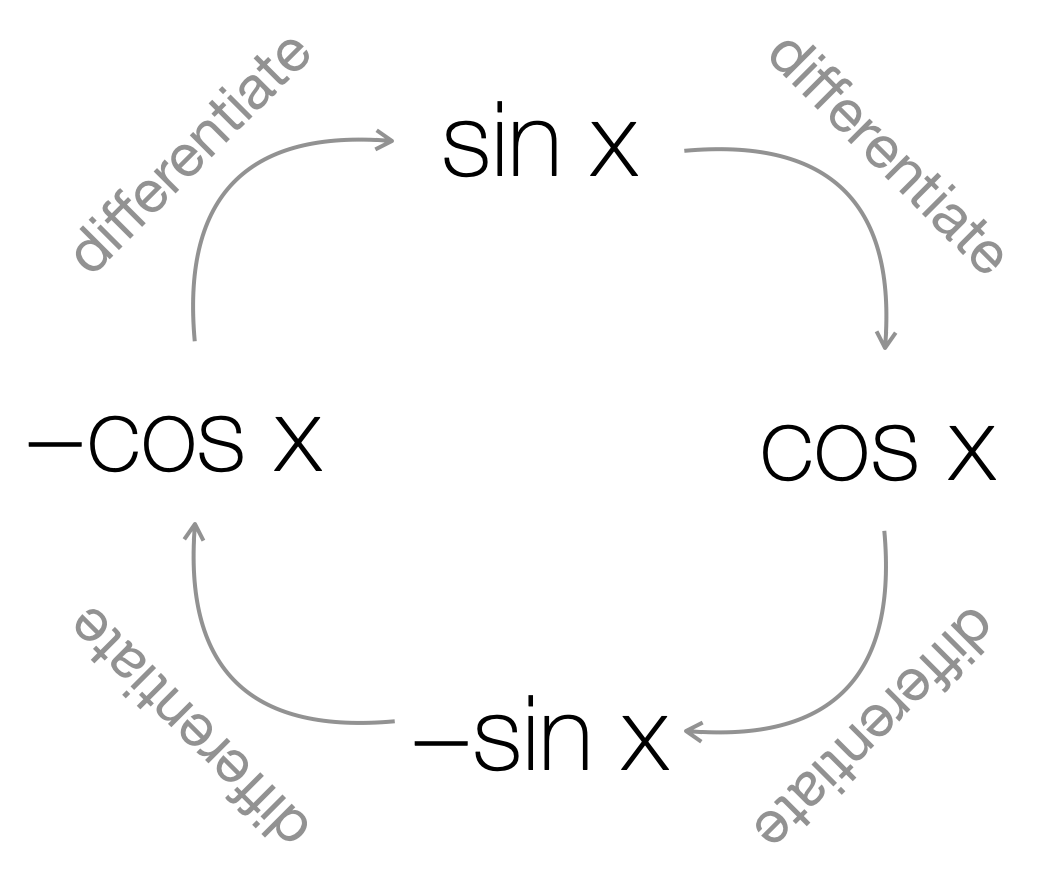
\includegraphics[width=0.6\linewidth]{images/difftrigcycle} 

}

\caption{The cycle of differentiation which links sin (x) and cos (x). sin (x) differentiates to cos (x), cos (x) differentiates to -sin (x), -sin (x) differentiates to -cos (x) and -cos (x) differentiates to sin x.}\label{fig:difftrig}
\end{figure}

\begin{equation}
\begin{array}{ccc}
  f(x) \equiv y & & f^{\prime}(x) \equiv \dfrac{\textrm{d}y}{\textrm{d}x}\\
  \hline
\sin Ax & &A\cos Ax \\
\cos Ax & &-A\sin Ax \\
-\sin Ax & &-A\cos Ax \\
-\cos Ax & &A\sin Ax \\
\\
\end{array}
\end{equation}

The differential of \(\tan x\) is not shown, it is shown later in section \ref{subsec:productrule}, but it is a result that is rarely needed in chemistry.

\hypertarget{subsec:turningpoints}{%
\subsection{Determining turning points}\label{subsec:turningpoints}}

As we have seen previously (in sections \ref{subsec:diffpolynomial} and \ref{subsec:difftrig}) we have taken note of points where the gradient (of differential) of a function is zero. These points are referred to as \emph{turning points}; there are three types of turning point, maxima, minima, and points of inflection (figure \ref{fig:turningpoints}). A turning point occurs when \(\frac{\textrm{d}y}{\textrm{d}x}\).

\begin{figure}

{\centering 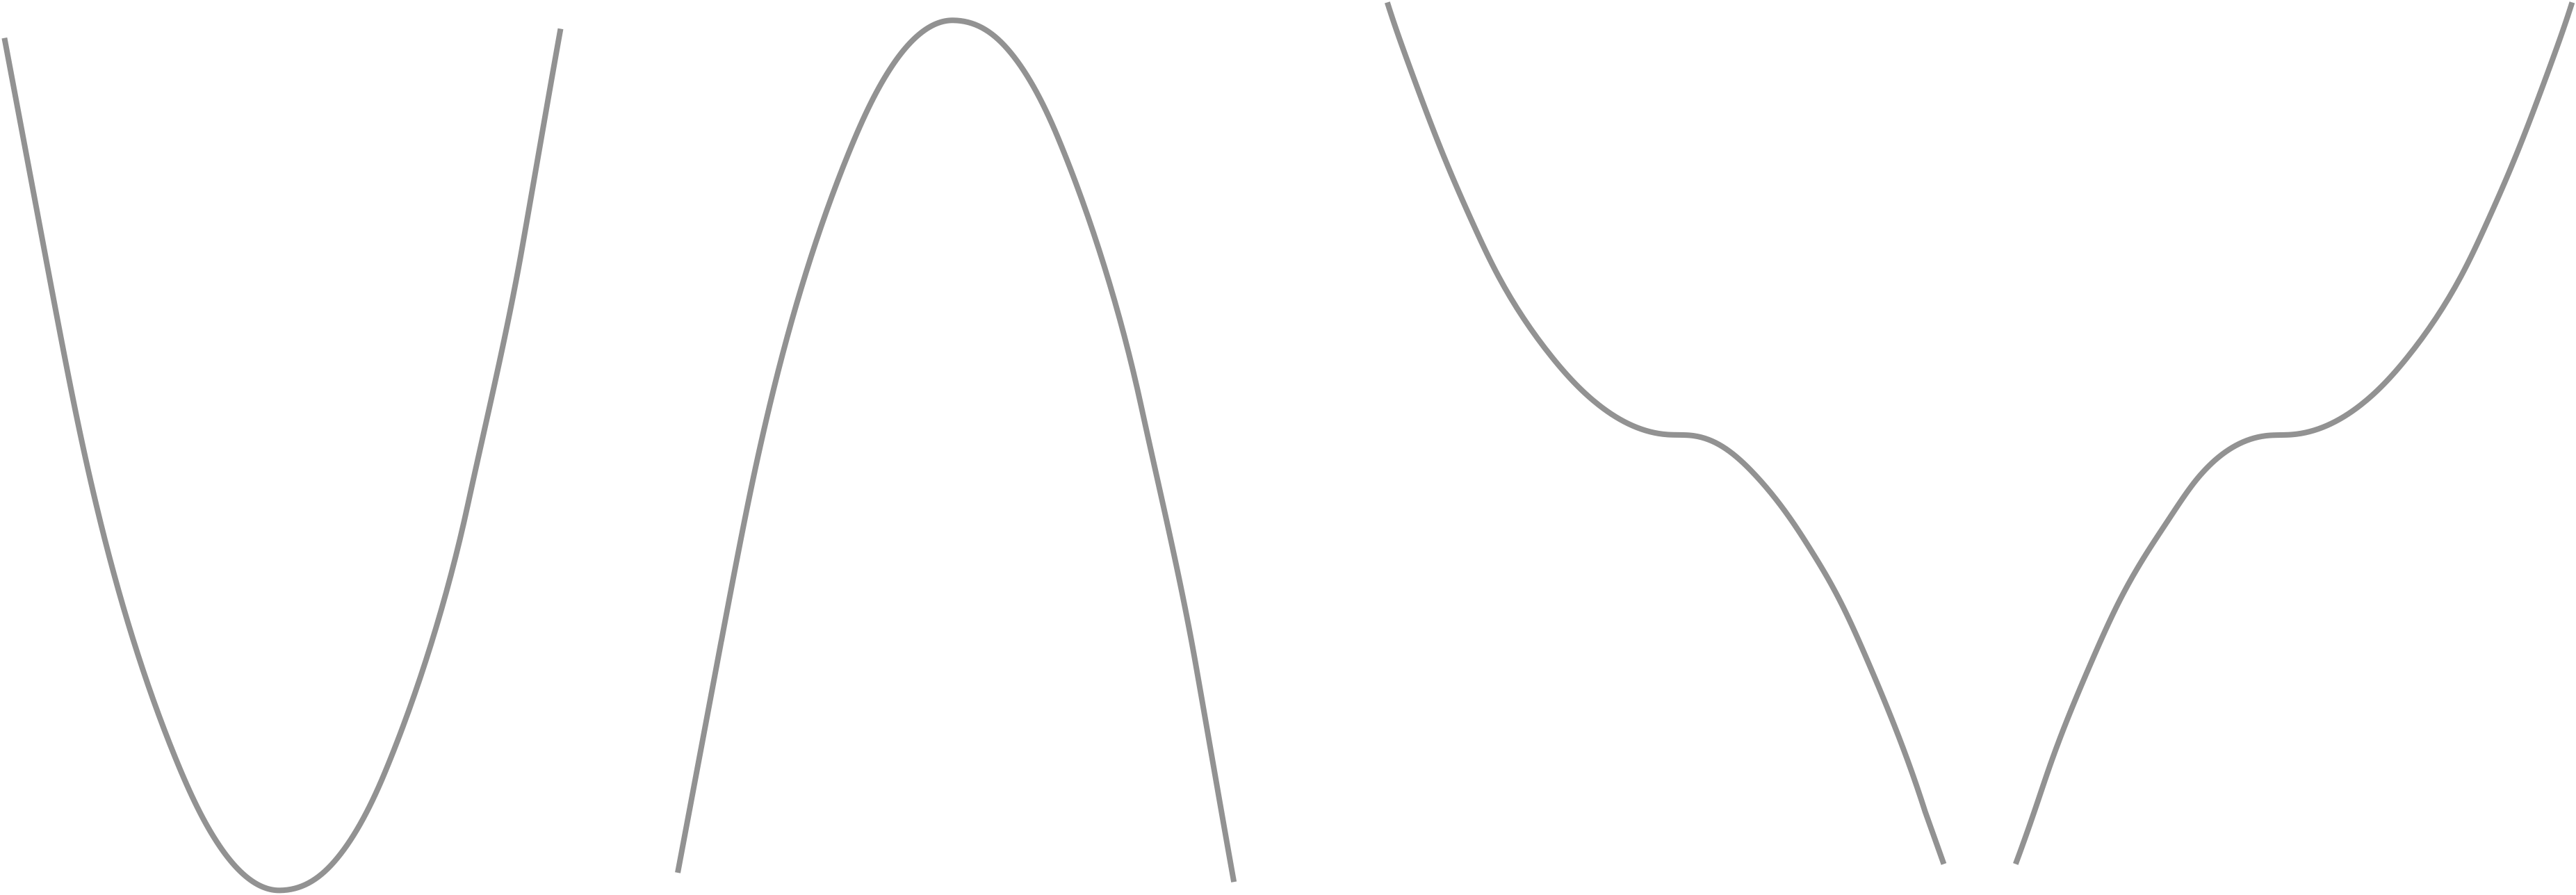
\includegraphics[width=0.6\linewidth]{images/turningpoints} 

}

\caption{The different types of turning point, from left: minima - a negative gradient which changes into a postive gradient, maxima - a postive gradient which changes into a negative gradient, and points of inflection which may either be postive gradients leveling to a zero gradient and increasing again, or negative gradients leveling to zero and decreasing again.}\label{fig:turningpoints}
\end{figure}

We can tell the nature of a turning point by one of two methods, first by inspection, and secondly using calculus and the second derivative of the function.

\hypertarget{determining-turning-points-by-inspection}{%
\subsubsection{Determining turning points by inspection}\label{determining-turning-points-by-inspection}}

The inspection method involves determining the coordinates of each turning point by differentiating the function. Then using the equation for the gradient of the line to include values just to the left and right of the turning point and determining if the gradient at that point is postive or negative.

For example, if we take the quadratic equation \(y=4x^2+3x-7\), and determine the differential of this function:

\begin{equation*}
\frac{\textrm{d}y}{\textrm{d}x} = 4x+3
\end{equation*}

At the turning point \(\dfrac{\textrm{d}y}{\textrm{d}x}=0\) and so at the turning point \(x=-\frac{3}{4}\). Now we can examine what value the gradient has if we choose, for example, values of \(x=-1\) and \(x=-\frac{1}{2}\).

At \(x=-1\), \(\frac{\textrm{d}y}{\textrm{d}x} = (4 \times -1)+3 = -1\), which is negative.

At \(x=-\frac{1}{2}\), \(\frac{\textrm{d}y}{\textrm{d}x} = (4 \times -\frac{1}{2})+3 = 1\), which is postive.

Therefore, a negative gradient which changes into a postive gradient with increasing value of x implies that this point is a \emph{minimum}.

It is adviseable to ensure points are close to the turning point of interest as some functions have more than one turning point.*

\hypertarget{determining-turning-points-by-differentiation}{%
\subsubsection{Determining turning points by differentiation}\label{determining-turning-points-by-differentiation}}

Our second method for determining the nature of a turning point is by determining the second derivative of the original function, \(\frac{\textrm{d}^2y}{\textrm{d}x^2}\). This second derivative is telling us the rate of change of the gradient.

If the second derivative is:
\begin{equation*}
\begin{array}{ccc}
  f'(x) \equiv \frac{\textrm{d}y}{\textrm{d}x} & & type of turning point\\
  \hline
\textrm{negative}  & & \textrm{maximum}\\
\textrm{positive} & & \textrm{minimum}\\
0 & & \textrm{point of inflection}\\
\end{array}
\end{equation*}

The nature of the point of inflection will have to be determined by the inspection method.

If we differentiate our function for a second time, and again input the value of x at the turning point, then we can tell the nature of the turning point.

If we use the same example as above:

\(y=4x^2+3x-7\), and \(\frac{\textrm{d}y}{\textrm{d}x} = 4x+3\), we can determine the second differential (\(\frac{\textrm{d}^2y}{\textrm{d}x^2}\)):

\begin{equation*}
\frac{\textrm{d}^2y}{\textrm{d}x^2} = 4
\end{equation*}

This second derivative is postive, and therefore we know that the turning point is a minimum.

\hypertarget{differentiating-functions-with-more-than-one-term}{%
\subsection{Differentiating functions with more than one term}\label{differentiating-functions-with-more-than-one-term}}

When differentiating functions with more than one term, we can just differentiate each term in turn. This is only true for when functions are added or subtracted. There are different rules for when two terms are multiplied by each other (the product rule - section \ref{subsec:productrule}) or when we have a function of a function (the chain rule \ref{subsec:chainrule}).

I have previously used differentiating \(y= \ln ax\) with respect to \(x\) as an example, and said that we can use our rules of logs to rearrange this to two terms, \(y= \ln a + \ln x\), when we differentiate this function we differentiate each term in tern.

Differentiating \(y=\ln a\), \(a\) is a constant, and so \(\frac{\textrm{d}y}{\textrm{d}x}=0\).

Differentiating \(y = \ln x\), \(\frac{\textrm{d}y}{\textrm{d}x}=\frac{1}{x}\).

Putting all of this together, \(\frac{\textrm{d}y}{\textrm{d}x}=0+ \frac{1}{x}= \frac{1}{x}\), the result I shared in section \ref{subsec:difflogs}.

Formally where \(y\) is a function of \(u\) \& \(v\), with each terms \(u(x)\) and \(v(x)\) being separate functions of \(x\), \(y = Au(x) + Bv(x)\), then \(\frac{\textrm{d}y}{\textrm{d}x}=A\frac{\textrm{d}u(x)}{\textrm{d}x} + B\frac{\textrm{d}v(x)}{\textrm{d}x}\).

\hypertarget{examples-1}{%
\section{Examples}\label{examples-1}}

During these examples (and during the questions below) a range of variables have been used because it is rare to meet examples in chemistry using \(x\) and \(y\). The principles are all the same, you are differentiating a dependent variable with respect to an independent variable.

\hypertarget{subsec:exdiffconsts}{%
\subsection{Differentiating constants}\label{subsec:exdiffconsts}}

Anything which isn't the variable we are differentitating with respect to may be considered a constant.

Determine \(\frac{\textrm{d}a}{\textrm{d}b}\) of the following function:

\begin{equation*}
a = 4x^3 + 3x^2 + 2x + 1
\end{equation*}

Since none of these terms contain the variable \(b\), these are all constants when differentiating this function with respect to \(b\).

Therefore \(\frac{\textrm{d}a}{\textrm{d}b}=0\)

\hypertarget{subsec:exdiffpoly}{%
\subsection{Differentiating polynomials}\label{subsec:exdiffpoly}}

Determine \(\frac{\textrm{d}a}{\textrm{d}b}\) of the following function:

\begin{equation*}
a = 4b^3 + 3b^2 - 2b + 1
\end{equation*}

We can differentiate each of these terms in turn:

\(\frac{\textrm{d}}{\textrm{d}b}4b^3 = 3 \times 4b^{3-1}= 12b^2\)

\(\frac{\textrm{d}}{\textrm{d}b}3b^2 = 2 \times 3b^{2-1}= 6b\)

\(\frac{\textrm{d}}{\textrm{d}b}(-2b) = 1 \times -2b^{1-1}= -2b^0 = -2\)

\(\frac{\textrm{d}}{\textrm{d}b}1 = 0\)

Therefore, putting each of these terms together: \(\frac{\textrm{d}a}{\textrm{d}b}=12b^2+6b-2\)

\hypertarget{subsec:exdiffexp}{%
\subsection{Differentiating exponentials}\label{subsec:exdiffexp}}

\hypertarget{subsec:exdifflogs}{%
\subsection{Differentiating logs}\label{subsec:exdifflogs}}

\hypertarget{subsec:exdifftrig}{%
\subsection{Differentiating trig functions}\label{subsec:exdifftrig}}

\hypertarget{subsec:exturningpoints}{%
\subsection{Determining turning points}\label{subsec:exturningpoints}}

The Lennard-Jones potential (figure \ref{fig:lennardjones}) describes the potential between two molecules, of which there is an equilibrium separation (\(r_{eq}\)) at the minimum of the function.

\begin{figure}

{\centering 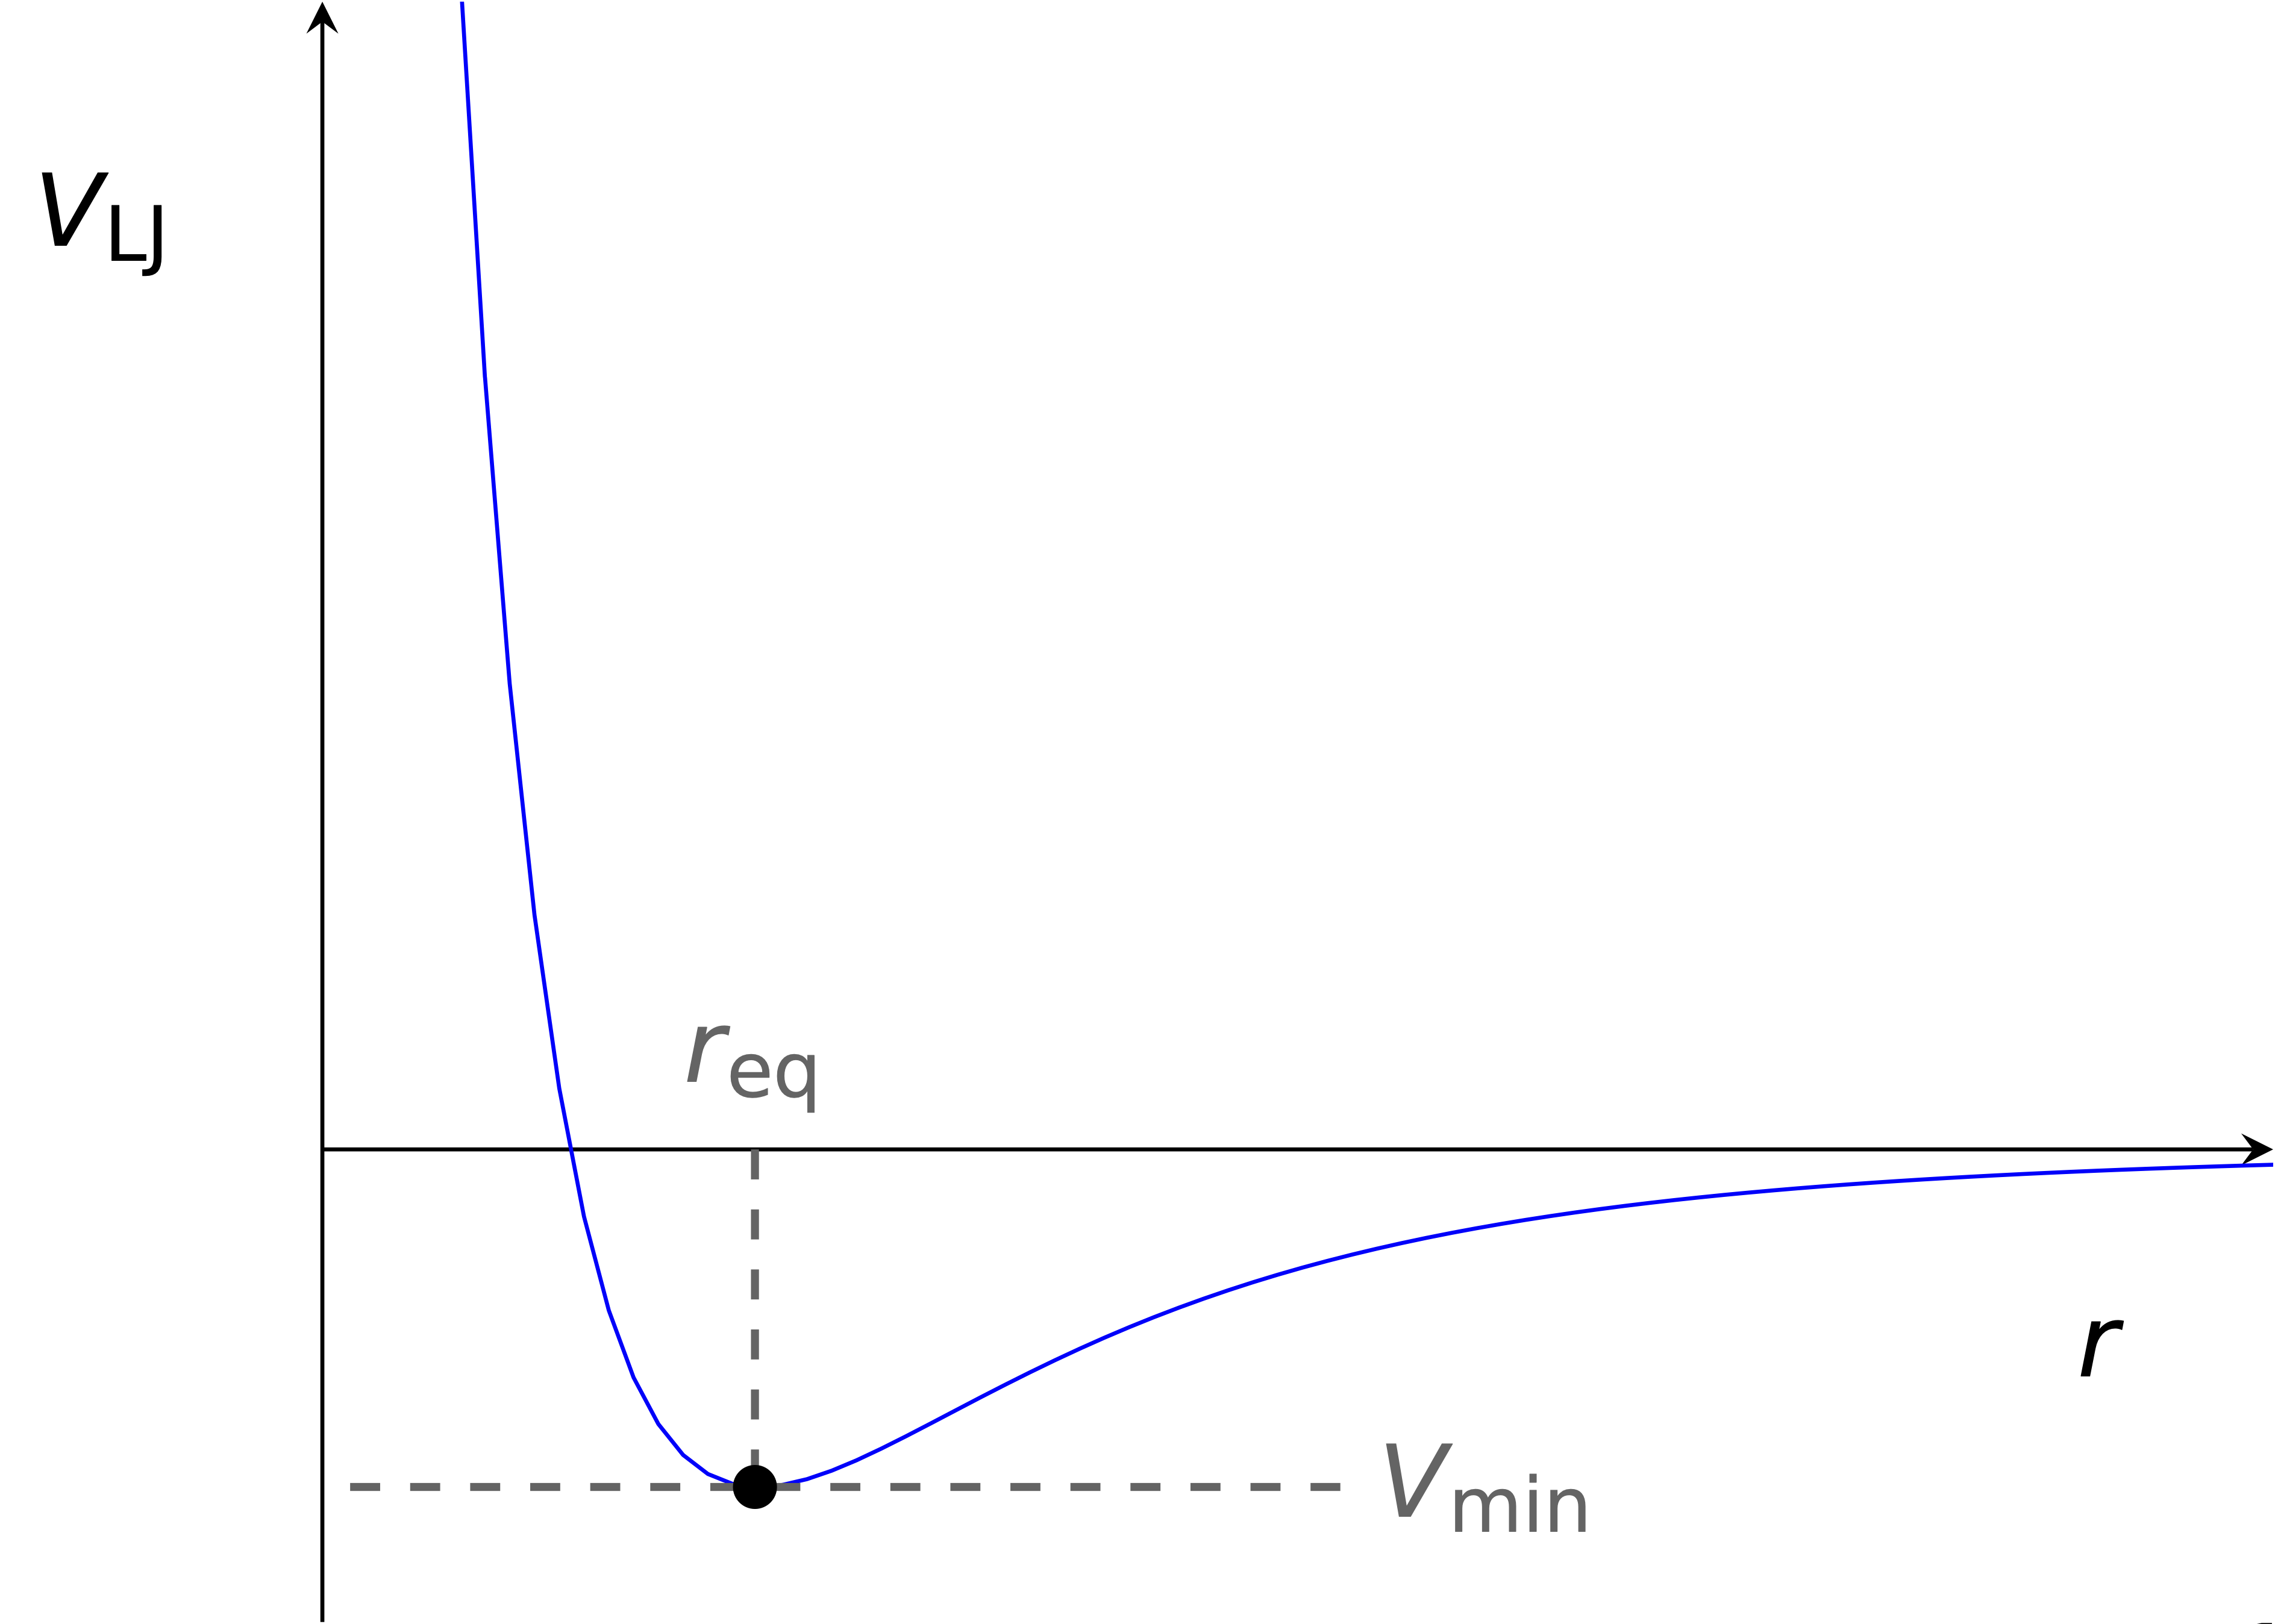
\includegraphics[width=0.4\linewidth]{images/lennardjones} 

}

\caption{The Lennard-Jones potential.}\label{fig:lennardjones}
\end{figure}

\hypertarget{summary-of-concepts-learnt-1}{%
\section{Summary of concepts learnt}\label{summary-of-concepts-learnt-1}}

\begin{equation*}
\begin{array}{ccc}
  f(x) \equiv y & & f^{\prime}(x) \equiv \dfrac{\textrm{d}y}{\textrm{d}x}\\
  \hline
A & &0 \\
 Ax^n & &nAx^{n-1} \\
 \dfrac{A}{x^n} \equiv A x^{-n} & &-nA x^{-n-1} \\
e^{Ax} & &Ae^{Ax} \\
A \ln Bx & &\dfrac{A}{x} \\
\sin Ax & &A\cos Ax \\
\cos Ax & &-A\sin Ax \\
\tan Ax & &-A\sec^2 Ax \\
\\
Au(x) + Bv(x) & &A\dfrac{\textrm{d}u(x)}{\textrm{d}x} + B\dfrac{\textrm{d}v(x)}{\textrm{d}x} \\
\end{array}
\end{equation*}

\hypertarget{sec:Questions4}{%
\section{Questions}\label{sec:Questions4}}

\hypertarget{simple-differentiation}{%
\subsection{`Simple' differentiation}\label{simple-differentiation}}

\begin{enumerate}
\def\labelenumi{\arabic{enumi}.}
\tightlist
\item
  Find \(\dfrac{\textrm{d}y}{\textrm{d}x}\) of the following functions:
\end{enumerate}

\begin{enumerate}
\def\labelenumi{\alph{enumi}.}
\tightlist
\item
  \(y = 6x + 4\)
\item
  \(y = 5x^2+ 3x-7\)
\item
  \(y = x^{-\frac{1}{2}}+ 3x-4\)
\item
  \(6x^{\frac{2}{3}}-x+9\)
\end{enumerate}

\begin{enumerate}
\def\labelenumi{\arabic{enumi}.}
\setcounter{enumi}{1}
\tightlist
\item
  Find \(\dfrac{\textrm{d}y}{\textrm{d}x}\) of the following functions:
\end{enumerate}

\begin{enumerate}
\def\labelenumi{\alph{enumi}.}
\tightlist
\item
  \(y = 3x^2 + \cos x\)
\item
  \(y = 6 \ln 2x\)
\item
  \(y = \frac{2}{3}e^{\frac{3x}{2}}\)
\item
  \(y = -e^{-5x}-e^{5x}\)
\end{enumerate}

\hypertarget{turning-points}{%
\subsection{Turning points}\label{turning-points}}

Find the turning points \((x,y)\) for the following functions:

\begin{enumerate}
\def\labelenumi{\arabic{enumi}.}
\tightlist
\item
  \(y = 2x^3 - 9x^2 + 12x\)
\item
  \(y = 12x^5 - 45x^4 + 40x^3\)
\end{enumerate}

\hypertarget{applied-questions}{%
\subsection{Applied questions}\label{applied-questions}}

\begin{enumerate}
\def\labelenumi{\arabic{enumi}.}
\tightlist
\item
  If two electric dipoles are aligned in an adjacent parallel manner such that they are separated by distance r, their potential energy of interaction, V, is given by:
\end{enumerate}

\begin{equation*}
V = \frac{\mu_1 \mu_2}{4 \pi \varepsilon_0 r^3}
\end{equation*}

determine \(\dfrac{\textrm{d}V}{\textrm{d}r}\)

\begin{enumerate}
\def\labelenumi{\arabic{enumi}.}
\setcounter{enumi}{1}
\tightlist
\item
  Light is scattered as it passes though solutions containing small particles with an intensity I, given by the following expression:
\end{enumerate}

\begin{equation*}
I = I_0 \frac{\pi \alpha ^2}{\varepsilon _r^2 \lambda^4 r^2})(\sin \phi)^2
\end{equation*}

determine expressions for how the intensity varies with:

\begin{enumerate}
\def\labelenumi{\alph{enumi}.}
\tightlist
\item
  wavelength, λ
\item
  angle, ϕ
\item
  distance from scatterer, r
\end{enumerate}

\emph{formally these are partial derivatives and we will learn about them next week in section \ref{subsec:partial}}

\begin{enumerate}
\def\labelenumi{\arabic{enumi}.}
\setcounter{enumi}{2}
\tightlist
\item
  The radius of a spherical balloon is increasing at a rate of 0.2 m s\textsuperscript{−1}. Find the rate of increase of (a) the volume and (b) the surface area of the balloon at the instant when the radius is 1.6 m.
\end{enumerate}

\hypertarget{sec:Answers4}{%
\section{Answers}\label{sec:Answers4}}

\hypertarget{simple-differentiation-1}{%
\subsection{`Simple' differentiation}\label{simple-differentiation-1}}

\begin{enumerate}
\def\labelenumi{\arabic{enumi}.}
\tightlist
\item
  \(\dfrac{\textrm{d}y}{\textrm{d}x}=\)
\end{enumerate}

\begin{enumerate}
\def\labelenumi{\alph{enumi}.}
\tightlist
\item
  6
\item
  \(10x+3\)
\item
  \(-\frac{1}{2}x{-\frac{3}{2}}+3\)
\item
  \(4x^{-\frac{1}{3}}-1\)
\end{enumerate}

\begin{enumerate}
\def\labelenumi{\arabic{enumi}.}
\setcounter{enumi}{1}
\tightlist
\item
  \(\dfrac{\textrm{d}y}{\textrm{d}x}=\)
\end{enumerate}

\begin{enumerate}
\def\labelenumi{\alph{enumi}.}
\tightlist
\item
  \(6x-\sin x\)
\item
  \(\frac{6}{x}\)
\item
  \(e^{\frac{3x}{2}}\)
\item
  \(5e^{-5x}-5e^{5x}\)
\end{enumerate}

\hypertarget{turning-points-1}{%
\subsection{Turning points}\label{turning-points-1}}

\begin{enumerate}
\def\labelenumi{\arabic{enumi}.}
\tightlist
\item
  (1,5)max, (2,4)min
\item
  (0,0) POI(+/+), (1,7)max, (2, −16)min
\end{enumerate}

\hypertarget{applied-questions-1}{%
\subsection{Applied questions}\label{applied-questions-1}}

\begin{enumerate}
\def\labelenumi{\arabic{enumi}.}
\item
  \begin{equation*}
  V = \frac{-3 \mu_1 \mu_2}{4 \pi \varepsilon_0 r^4}
  \end{equation*}
\item
  \begin{itemize}
  \item
  \end{itemize}
\end{enumerate}

\begin{enumerate}
\def\labelenumi{\alph{enumi}.}
\tightlist
\item
  \begin{equation*}
  \dfrac{\textrm{d}I}{\textrm{d}\lambda}= -4I_0 \frac{\pi \alpha ^2}{\varepsilon _r^2 \lambda^5 r^2}(\sin \phi)^2
  \end{equation*}
\item
  \begin{equation*}
  \dfrac{\textrm{d}I}{\textrm{d}\phi}= 2I_0 \frac{\pi \alpha ^2}{\varepsilon _r^2 \lambda^4 r^2}(\sin \phi)(\cos \phi)
  \end{equation*}
\item
  \begin{equation*}
  \dfrac{\textrm{d}I}{\textrm{d}r}= -2I_0 \frac{\pi \alpha ^2}{\varepsilon _r^2 \lambda^4 r^3}(\sin \phi)^2
  \end{equation*}
\end{enumerate}

\begin{enumerate}
\def\labelenumi{\arabic{enumi}.}
\setcounter{enumi}{2}
\tightlist
\item
  \(\dfrac{\textrm{d}V}{\textrm{d}t}= 0.8 \pi r^2\), \(\dfrac{\textrm{d}SA}{\textrm{d}t}=1.6 \pi r\)
\end{enumerate}

\hypertarget{ch:Workshop5}{%
\chapter{Week 5}\label{ch:Workshop5}}

\hypertarget{sec:Prelim5}{%
\section{Preliminary infomation}\label{sec:Prelim5}}

A recap of standard differentials\ldots{}

\begin{equation*}
\begin{array}{ccc}
  f(x) \equiv y & & f^{\prime}(x) \equiv \dfrac{\textrm{d}y}{\textrm{d}x}\\
  \hline
A & &0 \\
 Ax^n & &nAx^{n-1} \\
 \dfrac{A}{x^n} \equiv A x^{-n} & &-nA x^{-n-1} \\
e^{Ax} & &Ae^{Ax} \\
A \ln Bx & &\dfrac{A}{x} \\
\sin Ax & &A\cos Ax \\
\cos Ax & &-A\sin Ax \\
\tan Ax & &-A\sec^2 Ax \\
Au + Bv & &A\dfrac{\textrm{d}u}{\textrm{d}x} + B\dfrac{\textrm{d}v}{\textrm{d}x} \\
\end{array}
\end{equation*}

\hypertarget{subsec:chainrule}{%
\subsection{The Chain Rule}\label{subsec:chainrule}}

If differentiating a function of a function we use the `Chain Rule':

\(\dfrac{\textrm{d}y}{\textrm{d}x}=\dfrac{\textrm{d}y}{\textrm{d}u} \times \dfrac{\textrm{d}u}{\textrm{d}x}\)

\hypertarget{subsec:productrule}{%
\subsection{The Product Rule}\label{subsec:productrule}}

If differentiate a function times a function we use the `Product Rule', if :

\begin{equation*}
y= uv
\end{equation*}

\ldots where \(u\) and \(v\) are different functions of \(x\). The first derivative of this compound function may be found using the general differential form for products:

\begin{equation}
\textrm{d}(uv) = v\textrm{d}u + u\textrm{d}v
\label{eq:productrule}
\end{equation}

\hypertarget{subsec:partial}{%
\subsection{Partial differentiation}\label{subsec:partial}}

Any good scientist knows that you should only change one variable at a time to understand the effect it has on a system. This is exactly what partial differentiation does, although it recognises that there may be more than one variable in the system\ldots{}

Partial differentiation uses a different notation to standard differentiation to denote there is more than one variable. Subscritps are used to denote variables which are kept constant.

If y is a function of both x and z, then we can differentiate with respect to either variable, in this case we treat the other variable as a constant and differentiate as we ever have. The notation for differentiating y with respect to z as x is kept constant would be:

\begin{equation*}
\left(\frac{\partial y}{\partial z}\right)_x
\end{equation*}

In some circumstances you may wish to differentiate a function first by one variable and then by another, the notation is this case is:

\begin{equation*}
\left(\frac{\partial^2 y}{\partial x \partial z}\right)
\end{equation*}

this is implying that the partial derivative of y with respect to x was determined first and then the partial derivate of that first derivative was determined with respect to z. It should not matter in which order you perform these functions, they should both yield the same answer.

\hypertarget{sec:Questions5}{%
\section{Questions}\label{sec:Questions5}}

\hypertarget{chain-rule}{%
\subsection{Chain rule}\label{chain-rule}}

Find the turning points \((x,y)\) for the following functions:

\begin{enumerate}
\def\labelenumi{\arabic{enumi}.}
\tightlist
\item
  \(y = sin^2(x)\)
\item
  \(y = sin(e^{4x})\)
\item
  \(y = e^{(7x^2 + 2x)}\)
\item
  \(y = (x-1)^9\)
\end{enumerate}

\hypertarget{product-rule-questions}{%
\subsection{Product rule questions}\label{product-rule-questions}}

Differentiate the following using the product rule:

\begin{enumerate}
\def\labelenumi{\arabic{enumi}.}
\tightlist
\item
  \(y = x e^{7x}+ 7xe^x\)
\item
  \(y = 5x \cos (2x)\)
\item
  \(y = \frac{\sin x}{x^2}\)
\item
  \(y = \tan x\)
\end{enumerate}

\hypertarget{more-complex-differentiation-questions}{%
\subsection{More complex differentiation questions}\label{more-complex-differentiation-questions}}

Differentiate the following (you will need to decide if you need the product rule or the chain rule):

\begin{enumerate}
\def\labelenumi{\arabic{enumi}.}
\tightlist
\item
  \(y = x \ln x\)
\item
  \(y = \sin ^7 (5x)+ \cos ^5 (7x)\)
\item
  \(y = x^2 e^{x^2}\)
\item
  \(y = e^{\sin x^2}\)
\end{enumerate}

\hypertarget{partial-differentiation-questions}{%
\subsection{Partial differentiation questions}\label{partial-differentiation-questions}}

For the following function determine:

\(\left(\frac{\partial y}{\partial z}\right)_x\), \(\left(\frac{\partial y}{\partial x}\right)_z\), \(\left(\frac{\partial^2 y}{\partial z^2}\right)_x\), \(\left(\frac{\partial^2 y}{\partial x^z}\right)_z\), \(\left(\frac{\partial^2 y}{\partial x \partial z}\right)\) and \(\left(\frac{\partial^2 y}{\partial z \partial x}\right)\)

\begin{enumerate}
\def\labelenumi{\arabic{enumi}.}
\tightlist
\item
  \(y = x^6z -3x^2z^3+x^2z+6z^6+5\)
\item
  \(y = e^{3x}+ze^{2x}+x^2e^{-z}-z^2\)
\item
  \(y=\frac{\sin (3z)}{x}-\frac{1}{e^{3x}z^2}\)
\item
  \(y=\sin(3z^2+2xz+x^2)\)*
\end{enumerate}

*this one is involved - it uses both the chain and the product rule!

\hypertarget{sec:Answers5}{%
\section{Answers}\label{sec:Answers5}}

\hypertarget{chain-rule-1}{%
\subsection{Chain rule}\label{chain-rule-1}}

\begin{enumerate}
\def\labelenumi{\arabic{enumi}.}
\tightlist
\item
  \(\dfrac{\textrm{d}y}{\textrm{d}x}= 2 \sin x \cos x\)
\item
  \(\dfrac{\textrm{d}y}{\textrm{d}x}=4e^{4x}\cos (e^{4x})\)
\item
  \(\dfrac{\textrm{d}y}{\textrm{d}x}= (14x+2)e^{(7x^2 + 2x)}\)
\item
  \(\dfrac{\textrm{d}y}{\textrm{d}x}= 9 (x-1)^8\)
\end{enumerate}

\hypertarget{product-rule-questions-1}{%
\subsection{Product rule questions}\label{product-rule-questions-1}}

\begin{enumerate}
\def\labelenumi{\arabic{enumi}.}
\tightlist
\item
  \(\dfrac{\textrm{d}y}{\textrm{d}x}=e^{7x}+7xe^{7x}+ 7e^x+7xe^x\)
\item
  \(\dfrac{\textrm{d}y}{\textrm{d}x}=5 \cos (2x)-10x \sin (2x)\)
\item
  \(\dfrac{\textrm{d}y}{\textrm{d}x}= \frac{\cos x}{x^2}-\frac{2\sin x}{x^3}\)
\item
  \(\dfrac{\textrm{d}y}{\textrm{d}x}=\frac{1}{\cos^2 x}\)
\end{enumerate}

\hypertarget{more-complex-differentiation-questions-1}{%
\subsection{More complex differentiation questions}\label{more-complex-differentiation-questions-1}}

\begin{enumerate}
\def\labelenumi{\arabic{enumi}.}
\tightlist
\item
  \(\dfrac{\textrm{d}y}{\textrm{d}x}=\ln x +1\)
\item
  \(\dfrac{\textrm{d}y}{\textrm{d}x}=35 \cos (5x) \sin^6 (5x) - 35 \sin (7x) \cos^4(7x)\)
\item
  \(\dfrac{\textrm{d}y}{\textrm{d}x}=2x e^{x^2}+ 2x^3e^{x^2}\)
\item
  \(y=2x \cos x^2 e^{\sin x^2}\)
\end{enumerate}

\hypertarget{partial-differentiation-questions-1}{%
\subsection{Partial differentiation questions}\label{partial-differentiation-questions-1}}

\begin{enumerate}
\def\labelenumi{\arabic{enumi}.}
\item
  \(\left(\frac{\partial y}{\partial z}\right)_x= x^6-9x^2z^2+x^2+36z^5\),
  \(\left(\frac{\partial y}{\partial x}\right)_z=6x^5z-6xz^3+2xz\),
  \(\left(\frac{\partial^2 y}{\partial z^2}\right)_x=-18X^2z+180z^4\),
  \(\left(\frac{\partial^2 y}{\partial x^z}\right)_z=30x^4z-6z^3\),
  \(\left(\frac{\partial^2 y}{\partial x \partial z}\right)=6x^5-18xz^2+2x\) and
  \(\left(\frac{\partial^2 y}{\partial z \partial x}\right)=6x^5-18xz^2+2x\)
\item
  \(\left(\frac{\partial y}{\partial z}\right)_x=e^{2x}-x^2e^{-z}-2z\),
  \(\left(\frac{\partial y}{\partial x}\right)_z=3e^{3x}+2e^{2x}z+2xe^{-z}\),
  \(\left(\frac{\partial^2 y}{\partial z^2}\right)_x=x^2e^{-z}-2\),
  \(\left(\frac{\partial^2 y}{\partial x^z}\right)_z=9e^{3x}+4e^{2x}z+ 2e^{-z}\),
  \(\left(\frac{\partial^2 y}{\partial x \partial z}\right)=2e^{2x}-2xe^{-z}\) and
  \(\left(\frac{\partial^2 y}{\partial z \partial x}\right)=2e^{2x}-2xe^{-z}\)
\item
  \(\left(\frac{\partial y}{\partial z}\right)_x=\frac{\cos (3z)}{x}+\frac{2}{e^{3x}z^3}\),
  \(\left(\frac{\partial y}{\partial x}\right)_z=-\frac{\sin (3z)}{x^2}+\frac{3}{e^{3x}z^2}\),
  \(\left(\frac{\partial^2 y}{\partial z^2}\right)_x=-9\frac{\sin (3z)}{x}-\frac{6}{e^{3x}z^4}\),
  \(\left(\frac{\partial^2 y}{\partial x^z}\right)_z=\frac{2\sin (3z)}{x^3}-\frac{9}{e^{3x}z^2}\),
  \(\left(\frac{\partial^2 y}{\partial x \partial z}\right)=\frac{-3\cos (3z)}{x^2}-\frac{6}{e^{3x}z^3}\) and
  \(\left(\frac{\partial^2 y}{\partial z \partial x}\right)=\frac{-3\cos (3z)}{x^2}-\frac{6}{e^{3x}z^3}\)
\item
  \(\left(\frac{\partial y}{\partial z}\right)_x=(6z+2x)\cos(3z^2+2xz+x^2)\),
  \(\left(\frac{\partial y}{\partial x}\right)_z=(2z+2x)\cos(3z^2+2xz+x^2)\),
  \(\left(\frac{\partial^2 y}{\partial z^2}\right)_x=2\cos(3z^2+2xz+x^2)-(2z+2x)^2\sin(3z^2+2xz+x^2)\),
  \(\left(\frac{\partial^2 y}{\partial x^z}\right)_z=6\cos(3z^2+2xz+x^2)-(6z+2x)^2\sin(3z^2+2xz+x^2)\),
  \(\left(\frac{\partial^2 y}{\partial x \partial z}\right)=2\cos(3z^2+2xz+x^2)-(2z+2x)(6z+2x)\sin(3z^2+2xz+x^2)\) and
  \(\left(\frac{\partial^2 y}{\partial z \partial x}\right)=2\cos(3z^2+2xz+x^2)-(2z+2x)(6z+2x)\sin(3z^2+2xz+x^2)\) if you can do this one you can do them all!!!
\end{enumerate}

\hypertarget{ch:Workshop6}{%
\chapter{Week 6}\label{ch:Workshop6}}

\hypertarget{sec:Prelim6}{%
\section{Preliminary infomation}\label{sec:Prelim6}}

Standard anti derivatives (or integrals\ldots)

\begin{equation*}
\begin{array}{cccc}
f^{\prime}(x) \equiv y & & f(x) \equiv \int y ~\textrm{d}x & \textrm{Conditions}\\
  \hline
  \hline
A & & x + C \\ 
Ax^n & & \dfrac{A}{n+1}x^{n+1}+ C & x \neq -1\\ 
\dfrac{A}{x} \equiv A x^{-1} & &  A \ln x + C\\  
\dfrac{A}{Bx+ d} & & \dfrac{A}{B} \ln(Bx + d) +C\\ 
e^{Ax} & &\frac{1}{A} e^{Ax} + C\\
A^x && \frac{A^x}{\ln A} +C\\
A \ln x & & A \left( x \ln x - x \right)+ C\\

\sin Ax & &-\frac{1}{A}\cos Ax + C\\ 
\cos Ax & &\frac{1}{A}\sin Ax + C\\
\tan Ax & &-\frac{1}{A}\ln(\cos Ax) + C \equiv \frac{1}{A}\ln(\sec Ax) + C & -\frac{\pi}{2} < x < \frac{\pi}{2}\\

\frac{A}{x^2 + B^2} && \frac{A}{B}\tan^{-1}\left(\frac{x}{B}\right) + C &B>0\\
Ax^2 e^{Bx} && A\left(\frac{x^2}{B} - \frac{2x}{B^2} + \frac{2}{B^3} \right)e^{Bx} +C\\

v(x) \frac{\textrm{d}u(x)}{\textrm{d}x} && u(x)v(x) - \int u(x)\frac{\textrm{d}v(x)}{\textrm{d}x} +C & \textrm{Integration by Parts}\\

Au + Bv & &A\dfrac{\textrm{d}u}{\textrm{d}x} + B\dfrac{\textrm{d}v}{\textrm{d}x} \\
\end{array}
\end{equation*}

\hypertarget{sec:Questions6}{%
\section{Questions}\label{sec:Questions6}}

\hypertarget{basic-integration-practice}{%
\subsection{Basic integration practice}\label{basic-integration-practice}}

Integrate the following with respect to the variable specified:

\begin{enumerate}
\def\labelenumi{\arabic{enumi}.}
\tightlist
\item
  \(f'(x) = \frac{a}{x}\); x
\item
  \(f'(x) = x^\frac{3}{2}+ \frac{x^\frac{1}{2}}{2} - 2x^{-\frac{1}{2}}\), x
\item
  \(f'(b) = \sin (ab)\); b
\item
  \(f'(T) = a + bT + \frac{c}{T}\); T
\item
  \(f'(t) = k\); t
\item
  \(f'([A]) = \frac{1}{[A]}\), {[}A{]}
\item
  \(f'([A]) = \frac{1}{[A]^2}\), {[}A{]}
\item
  \(f'(t) = -e^{-kt}\), t
\end{enumerate}

\hypertarget{differential-equations}{%
\subsection{Differential equations}\label{differential-equations}}

Solve the following differential equations as far as possible:

\begin{enumerate}
\def\labelenumi{\arabic{enumi}.}
\tightlist
\item
  \(\frac{\textrm{d}\ln a}{\textrm{d}z}= bz^2\)
\item
  \(\frac{\textrm{d}[A]}{\textrm{d}t} = -k[A]^2\), when t= 0, {[}A{]} = {[}A{]}\textsubscript{0}
\item
  \(\frac{\textrm{d}p}{\textrm{d}T}=\frac{p\Delta_{\textrm{vap}}H}{RT^2}\); when T = T\textsubscript{1}, p = p\textsubscript{1} and when when T = T\textsubscript{2}, p = p\textsubscript{2}
\item
  \(\frac{\textrm{d}w}{\textrm{d}V}= -\frac{nRT}{V}\), when V = V\textsubscript{i}, w = 0 and when V = V\textsubscript{f}, w = w
\end{enumerate}

\hypertarget{sec:Answers6}{%
\section{Answers}\label{sec:Answers6}}

\hypertarget{basic-integration-practice-1}{%
\subsection{Basic integration practice}\label{basic-integration-practice-1}}

\begin{enumerate}
\def\labelenumi{\arabic{enumi}.}
\tightlist
\item
  \(f (x) = a \ln x + C\)
\item
  \(f(x) = \frac{2}{5} x^{\frac{5}{2}}+ \frac{x^{\frac{3}{2}}}{3}+4x^{\frac{1}{2}}+C\)
\item
  \(f(b) =-\frac{1}{a}\cos (ab) + C\)
\item
  \(f(T) = aT + \frac{bT^2}{2} + c\ln T + C\)
\item
  \(f(t) = kt +C\)
\item
  \(f([A])= \ln [A] + C\)
\item
  \(f([A])=-\frac{1}{[A]}+ C\)
\item
  \(f(t) = \frac{e^{-kt}}{k}\)
\end{enumerate}

\hypertarget{differential-equations-1}{%
\subsection{Differential equations}\label{differential-equations-1}}

\begin{enumerate}
\def\labelenumi{\arabic{enumi}.}
\tightlist
\item
  \(\ln a = \frac{bz^3}{3}+D\)
\item
  \(\frac{1}{[A]}=\frac{1}{[A]_0}+ kt\)
\item
  \(\ln \frac{p_1}{p_2}=\frac{\Delta_{\textrm{vap}}H}{R}\left({\frac{1}{T_2}-\frac{1}{T_1}}\right)\)
\item
  \(w = -nRT \ln \frac{V_f}{V_i}\)
\end{enumerate}

\hypertarget{ch:questions}{%
\chapter{Miscellaneous questions}\label{ch:questions}}

The following questions use skills you have learnt in this course. The skills you have learnt are no longer listed to make these more problem solving.

\hypertarget{questions}{%
\section{Questions}\label{questions}}

\begin{enumerate}
\def\labelenumi{\arabic{enumi}.}
\tightlist
\item
  Determine the average volume occupied by a single water molecule (in Å\textsuperscript{3}) given the density of water is 0.9982071 kg dm\textsuperscript{-3} at 20 ºC.
\end{enumerate}

\hypertarget{answers}{%
\section{Answers}\label{answers}}

\begin{enumerate}
\def\labelenumi{\arabic{enumi}.}
\tightlist
\item
  29.9688 Å\textsuperscript{3}
\end{enumerate}

\hypertarget{other-useful-infomation}{%
\chapter{Other useful infomation}\label{other-useful-infomation}}

\hypertarget{physical-constants}{%
\section{Physical constants}\label{physical-constants}}

\begin{longtable}[]{@{}cc@{}}
\caption{Physical constants used in this work\label{tab:physicalconst}}\tabularnewline
\toprule
\endhead
\(R\) & 8.31446261815324 J K\textsuperscript{-1} mol\textsuperscript{-1}\tabularnewline
\(N_A\) & 6.02214076 × 10\textsuperscript{23} mol\textsuperscript{-1}\tabularnewline
\(c\) & 299792458 m s\textsuperscript{-1}\tabularnewline
\(e\) & 1.60217653(14) × 10\textsuperscript{-19} C\tabularnewline
\bottomrule
\end{longtable}

The numbers in brackets refer to the error in the previous digits

\hypertarget{molar-masses}{%
\section{Molar masses}\label{molar-masses}}

\hypertarget{physical-constants-1}{%
\section{Physical constants}\label{physical-constants-1}}

\begin{longtable}[]{@{}cc@{}}
\caption{Physical constants used in this work\label{tab:physicalconst}}\tabularnewline
\toprule
Element or isotope & g mol\textsuperscript{-1}\tabularnewline
\midrule
\endfirsthead
\toprule
Element or isotope & g mol\textsuperscript{-1}\tabularnewline
\midrule
\endhead
H & 1.00794\tabularnewline
O & 15.9994\tabularnewline
\bottomrule
\end{longtable}

\hypertarget{sec:maclaurin}{%
\section{Maclaurin expansions of common functions}\label{sec:maclaurin}}

\hypertarget{subsec:macexp}{%
\subsection{Maclaurin expansion of exponential functions}\label{subsec:macexp}}

The function \(e^{ax}\) may be expressed as a series of polynomials:

\begin{equation}
e^{ax} = \frac{(ax)^0}{0!} + \frac{(ax)^1}{1!} + \frac{(ax)^2}{2!} + \frac{(ax)^3}{3!} + \dots + \frac{(ax)^\infty}{\infty!}
\label{eq:macexp}
\end{equation}

The factoral (\(!\)) notation used in equation \eqref{eq:macexp} is a shorthand way of expressing a series of multiplication. It is each positive integer up to that value multiplied together. For example \(5! = 5 \times 4 \times 3\times 2 \times 1\). \(0!=1\), why is explained in \href{https://www.youtube.com/watch?v=Mfk_L4Nx2ZI}{this video}.

Knowing the Maclaurin expansion for \(e^{ax}\) it becomes obvious why the differential of this function \(\frac{\textrm{d}}{\textrm{d}x}e^{ax}=ae^{ax}\). See section \ref{subsec:diffexp}.

\hypertarget{subsec:mactrig}{%
\subsection{Maclaurin expansion of trig functions}\label{subsec:mactrig}}

\begin{equation}
\sin(bx) = \frac{(bx)^1}{1!} - \frac{(bx)^3}{3!} + \frac{(bx)^5}{5!} - \frac{(bx)^7}{7!}  + \frac{(bx)^9}{9!} - \dots
\label{eq:macsin}
\end{equation}

\begin{equation}
\cos(cx) = \frac{(cx)^0}{0!} - \frac{(cx)^2}{2!} + \frac{(cx)^4}{4!} - \frac{(cx)^6}{6!}  + \frac{(cx)^8}{8!} - \dots
\label{eq:maccos}
\end{equation}

  \bibliography{book.bib,packages.bib}

\end{document}
